\chapter{Desarrollo Experimental y Análisis de Resultados}

En este capítulo se detallan los procedimientos experimentales realizados en el laboratorio para cada una de las
siete experiencias programadas en la consigna de la cátedra, presentando los circuitos de medición, los diagramas de
señal, los cuadros de datos medidos, las capturas oscilográficas y los cálculos correspondientes.

% =========================================================================
% EXPERIMENTO 1
% =========================================================================
\section{Experimento 1: Análisis de una Forma de Onda Cuadrada}
\label{sec.ej1:onda_cuadrada}

\subsection{Procedimiento y Circuito de Medición}
Se conectó la salida del generador de funciones ajustada en onda cuadrada simétrica ($f_0 = \qty{1}{\kilo\hertz}$, sin CC y nivel medio) a la entrada del osciloscopio digital mediante una sonda atenuadora X10 compensada, de acuerdo con el circuito de la Figura~\ref{crkt.ej1:medicion_cuadrada}.

\begin{figure}[!ht]
    \centering
    % Circuito de medición para el Experimento 1: Onda cuadrada con DSO
\begin{circuitikz}[scale=0.9, transform shape]
    % Generador de funciones
    \draw (0,0) node[ground] {}
        to[sV, l={$G_1$ (\qty{1}{\kilo\hertz})}] (0,2)
        to[short] (1.5,2);
    \draw (0,0) to[short] (1.5,0);

    % Conexión y sonda atenuadora 10X
    \draw (1.5,2) to[R, l={Sonda 10X}] (4.5,2)
        to[short, -o] (5.2,2) node[above, font=\scriptsize\bfseries] {CH1};
    \draw (1.5,0) to[short] (4.5,0)
        to[short, -o] (5.2,0) node[above, font=\scriptsize\bfseries] {Masa};

    % Conexiones al panel del instrumento
    \draw (5.2,2) to[short] (5.8,2);
    \draw (5.2,0) to[short] (5.8,0);
    \draw (5.2,0) node[ground] {};

    % Bloque osciloscopio DSO
    \draw[thick, rounded corners=3pt, fill=blue!3] (5.8,-0.8) rectangle (10.4,2.8);
    \node at (8.1,2.3) [font=\bfseries\small] {Osciloscopio DSO};
    \node at (8.1,1.55) [font=\scriptsize, align=center] {Acoplamiento CC / Sin límite BW};
    \node at (8.1,0.95) [font=\scriptsize, align=center] {Math: FFT / Ventana Flattop};
    \node at (8.1,0.35) [font=\scriptsize, align=center] {Adquisición: Promedio 64};

    % Cuadro TP Calibración
    \node[draw, dashed, rounded corners, font=\tiny, align=center, fill=gray!8] at (8.1,-0.35) 
        {TP Calibración (\qty{1}{\kilo\hertz}, \qty{5}{\volt_{pp}})};
\end{circuitikz}

    \caption{Circuito de conexión para la medición de la onda cuadrada con el osciloscopio digital.}
    \label{crkt.ej1:medicion_cuadrada}
\end{figure}

En la Figura~\ref{fig.ej1:tiempo_cuadrada} se presenta el oscilograma adquirido en el dominio del tiempo, donde se verifica una frecuencia fundamental de $\qty{1.000}{\kilo\hertz}$, tensión pico a pico de $\qty{10.4}{\volt}$ y un ciclo de trabajo del $50\%$.

\begin{figure}[!ht]
    \centering
    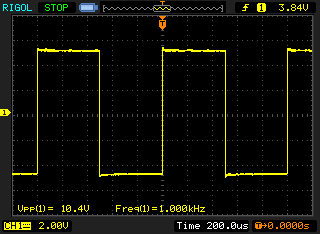
\includegraphics[width=0.46\textwidth]{pictures/NewFile0.png}
    \caption{Oscilograma temporal de la onda cuadrada en el osciloscopio digital ($f_0 = \qty{1.000}{\kilo\hertz}$, $V_{pp} = \qty{10.4}{\volt}$).}
    \label{fig.ej1:tiempo_cuadrada}
\end{figure}

\subsection{Observaciones de Adquisición y Ventanas}
Siguiendo la consigna, se realizaron las siguientes observaciones:
\begin{itemize}
    \item \textbf{Modo de Adquisición:} Al alternar entre los modos Normal, Detección de Pico y Promedio (con 64 cuentas),
    se constató que en modo Normal el piso de ruido fluctuó continuamente; en modo Pico el piso de ruido aparente se
    elevó al registrar valores extremos; mientras que en modo Promedio (64 cuentas) las fluctuaciones aleatorias del
    ruido se promediaron, dejando un trazo limpio y estable.
    \item \textbf{Tipo de Ventana:} Se alternó entre las ventanas disponibles en el osciloscopio (Rectangular, Hanning y Blackman). Se observó que la ventana Rectangular brindó la mayor resolución frecuencial con lóbulos laterales pronunciados; Hanning ofreció un menor derrame lateral; y Blackman proporcionó un marcado rechazo de lóbulos secundarios, facilitando la lectura de amplitud. Cabe aclarar que el instrumento empleado (Rigol DS1052E) no dispone de la ventana Flattop solicitada en la consigna, motivo por el cual se seleccionó Blackman en su sustitución.
\end{itemize}

\subsection{Mediciones de Frecuencia y Amplitud Armónica}
Con el modo de adquisición en Promedio (64 cuentas) y ventana Rectangular, se ingresó al menú Cursores (Tipo Frecuencia,
Fuente Matemática) determinando las frecuencias de las siete primeras componentes espectrales, registradas en el
Cuadro~\ref{tab.ej1:frecuencias}.

\begin{table}[!ht]
    \centering
    \resizebox{\textwidth}{!}{%
    \begin{tabular}{lccccccc}
        \toprule
        \textbf{Componente Espectral} & \textbf{1} & \textbf{2} & \textbf{3} & \textbf{4} & \textbf{5} & \textbf{6} & \textbf{7} \\
        \midrule
        Frecuencia med. [$f_n \pm U(f)$] [$\unit{\kilo\hertz}$] & $1{,}00 \pm 0{,}05$ & $3{,}00 \pm 0{,}05$ & $5{,}00 \pm 0{,}05$ & $7{,}00 \pm 0{,}05$ & $9{,}00 \pm 0{,}05$ & $11{,}00 \pm 0{,}05$ & $13{,}00 \pm 0{,}05$ \\
        Orden armónico ($n$) & 1° & 3° & 5° & 7° & 9° & 11° & 13° \\
        \bottomrule
    \end{tabular}}
    \caption{Frecuencias de las siete primeras componentes espectrales medidas en la onda cuadrada ($k=2$).}
    \label{tab.ej1:frecuencias}
\end{table}

Tal como se observa, únicamente se manifiestan armónicos impares ($1\,\unit{\kilo\hertz}$, $3\,\unit{\kilo\hertz}$,
$5\,\unit{\kilo\hertz}$, etc.), comprobándose la ausencia de componentes pares en la onda simétrica. En la
Figura~\ref{fig.ej1:espectro_experimental} se exponen las capturas espectrales registradas con el osciloscopio digital:
con ventana Rectangular (Figura~\ref{fig.ej1:fft_rect}) para la discriminación nítida de rayas y con ventana Blackman
(Figura~\ref{fig.ej1:fft_blackman}) empleada para la medición rigurosa de niveles en decibeles.

\begin{figure}[!ht]
    \centering
    \begin{subfigure}[t]{0.48\textwidth}
        \centering
        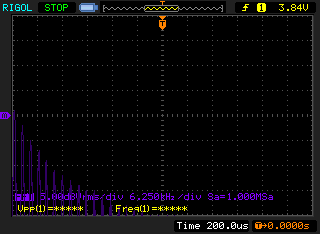
\includegraphics[width=\textwidth]{pictures/NewFile5.png}
        \caption{Ventana Rectangular (armónicos impares).}
        \label{fig.ej1:fft_rect}
    \end{subfigure}
    \hfill
    \begin{subfigure}[t]{0.48\textwidth}
        \centering
        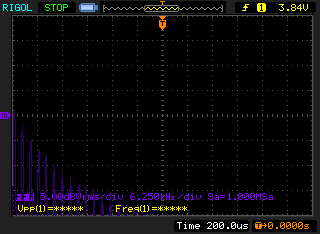
\includegraphics[width=\textwidth]{pictures/NewFile6.png}
        \caption{Ventana Blackman (medición de amplitudes).}
        \label{fig.ej1:fft_blackman}
    \end{subfigure}
    \caption{Espectro FFT experimental de la onda cuadrada en el osciloscopio digital.}
    \label{fig.ej1:espectro_experimental}
\end{figure}

A continuación, para la determinación de amplitudes, debido a que la ventana Flattop no se encuentra disponible en el osciloscopio Rigol DS1052E, se utilizó en su reemplazo la ventana Blackman de acuerdo con lo indicado en la guía de laboratorio (\emph{«Usamos blacman (Rigol DS105SE)»}). Con los cursores en Amplitud se midieron los niveles en decibeles respecto a un volt ($\unit{\dBV}$). Se calculó la tensión eficaz de cada armónico aplicando la expresión de la consigna:
\begin{equation}
    V_n = 10^{\frac{\text{dBv}}{20}} \quad [\unit{\volt}]
    \label{eq.ej1:conversion_dbv}
\end{equation}
Los valores obtenidos se presentan en el Cuadro~\ref{tab.ej1:amplitudes}.

\begin{table}[!ht]
    \centering
    \resizebox{\textwidth}{!}{%
    \begin{tabular}{lccccccc}
        \toprule
        \textbf{Componente Espectral} & \textbf{1} & \textbf{2} & \textbf{3} & \textbf{4} & \textbf{5} & \textbf{6} & \textbf{7} \\
        \midrule
        Tensión simbólica ($V$) & $V_1$ & $V_2$ & $V_3$ & $V_4$ & $V_5$ & $V_6$ & $V_7$ \\
        Nivel medido [$\unit{\dBV}$] & $10{,}0$ & $0{,}0$ & $-3{,}0$ & $-6{,}0$ & $-8{,}0$ & $-10{,}0$ & $-11{,}0$ \\
        $V = 10^{\frac{\text{dBv}}{20}}$ [$\unit{\volt}$] & $3{,}16$ & $1{,}00$ & $0{,}71$ & $0{,}50$ & $0{,}40$ & $0{,}32$ & $0{,}28$ \\
        $V^2$ [$\unit{\volt\squared}$] & $10{,}00$ & $1{,}00$ & $0{,}50$ & $0{,}25$ & $0{,}16$ & $0{,}10$ & $0{,}08$ \\
        \bottomrule
    \end{tabular}}
    \caption{Amplitudes armónicas y potencias cuadráticas medidas con ventana Blackman (reemplazo de Flattop no disponible).}
    \label{tab.ej1:amplitudes}
\end{table}

\subsection{Cálculo del Valor Eficaz y Comparación}
A partir de la sumatoria cuadrática de los armónicos medidos, se calculó el valor eficaz de la señal:
\begin{equation}
\begin{aligned}
    V_{\text{ef(calc)}} &= \sqrt{\sum_{n=1}^{7} V_n^2} \\
    &= \sqrt{10{,}00 + 1{,}00 + 0{,}50 + 0{,}25 + 0{,}16 + 0{,}10 + 0{,}08} \approx \qty{3.48 \pm 0.37}{\volt}
\end{aligned}
\label{eq.ej1:vef_calculado}
\end{equation}

Por su parte, la medición del valor eficaz efectuada con el instrumento arrojó:
\begin{equation}
    V_{\text{ef(medido)}} = \qty{4.94 \pm 0.15}{\volt}
    \label{eq.ej1:vef_medido}
\end{equation}

Al comparar ambas determinaciones, se constata que el valor obtenido por cálculo a partir de la FFT ($\qty{3.48}{\volt}$)
es menor que el valor medido sobre la forma de onda completa en el tiempo ($\qty{4.94}{\volt}$). Esta diferencia se debe
a que el cálculo espectral incorporó únicamente los primeros 7 armónicos impares (hasta $\qty{13}{\kilo\hertz}$); dado
que una onda cuadrada contiene armónicos impares que se extienden teóricamente hasta el infinito, la potencia de los
armónicos superiores no computados en la sumatoria explica por qué el valor eficaz calculado resulta inferior al medido.

% =========================================================================
% EXPERIMENTO 2
% =========================================================================
\section{Experimento 2: Análisis de un Tren de Pulsos}
\label{sec.ej2:tren_pulsos}

\subsection{Procedimiento y Circuito de Medición}
Mediante el control de simetría del generador de funciones (tirando de la perilla \texttt{Pull to Var - Ramp/Pulse}),
se ajustó la salida para obtener una forma de onda de pulsos con período $T = \qty{1}{\milli\second}$ y ancho de pulso
$t_0 = \qty{250}{\micro\second}$, manteniendo el nivel en media vuelta. La señal se conectó simultáneamente al canal CH1
del osciloscopio y a un multímetro digital dispuesto para medir tensión continua ($V_{\text{DC}}$), tal como se
esquematiza en la Figura~\ref{crkt.ej2:medicion_pulsos}.

\begin{figure}[!ht]
    \centering
    % Circuito de medición para el Experimento 2: Tren de pulsos con DSO y Multímetro True RMS
\begin{circuitikz}[scale=0.9, transform shape]
    % Generador de funciones
    \draw (0,0.5) node[ground] {}
        to[sV, l={$G_1$ (Pulsos)}] (0,2.5)
        to[short, -*] (2.2,2.5);
    \draw (0,0.5) to[short, -*] (2.2,0.5);

    % Derivación superior hacia el Osciloscopio DSO
    \draw (2.2,2.5) to[short] (2.2,2.2)
        to[short, -o] (4.8,2.2) node[above, font=\scriptsize\bfseries] {CH1};
    \draw (2.2,0.5) to[short] (2.2,1.0)
        to[short, -o] (4.8,1.0) node[above, font=\scriptsize\bfseries] {Masa};

    % Conexión al bloque DSO
    \draw (4.8,2.2) to[short] (5.4,2.2);
    \draw (4.8,1.0) to[short] (5.4,1.0);
    \draw (4.8,1.0) node[ground] {};

    % Bloque osciloscopio
    \draw[thick, rounded corners=3pt, fill=blue!3] (5.4,0.4) rectangle (10.0,2.9);
    \node at (7.7,2.5) [font=\bfseries\small] {Osciloscopio DSO};
    \node at (7.7,1.85) [font=\scriptsize, align=center] {CH1: FFT / Temporal\\Promedio 64 cuentas};
    \node at (7.7,1.1) [font=\scriptsize, align=center] {Ventanas: Flattop / Rect.\\Cursores de frecuencia y amplitud};

    % Derivación inferior hacia el Multímetro True RMS
    \draw (2.2,2.5) to[short] (2.2,-1.1)
        to[short, -o] (4.8,-1.1) node[above, font=\scriptsize\bfseries] {$V/\Omega$};
    \draw (2.2,0.5) to[short] (2.2,-1.9)
        to[short, -o] (4.8,-1.9) node[above, font=\scriptsize\bfseries] {COM};

    % Conexión al bloque Multímetro
    \draw (4.8,-1.1) to[short] (5.4,-1.1);
    \draw (4.8,-1.9) to[short] (5.4,-1.9);
    \draw (4.8,-1.9) node[ground] {};

    % Bloque Multímetro True RMS
    \draw[thick, rounded corners=3pt, fill=purple!5] (5.4,-2.5) rectangle (10.0,-0.6);
    \node at (7.7,-1.1) [font=\bfseries\small] {Multímetro Digital};
    \node at (7.7,-1.8) [font=\scriptsize, align=center] {UNI-T UT89X (Escala $V_{\text{DC}}$)\\Medición directa del valor medio};
\end{circuitikz}

    \caption{Circuito de conexión para el análisis del tren de pulsos con DSO y Multímetro True RMS.}
    \label{crkt.ej2:medicion_pulsos}
\end{figure}

En la Figura~\ref{fig.ej2:tiempo_pulsos} se expone el oscilograma adquirido en el dominio del tiempo, verificando
un período de $\qty{1.000}{\milli\second}$, ancho de pulso de $\qty{250}{\micro\second}$, valor eficaz de
$\qty{5.11}{\volt}$ y amplitud pico a pico de $\qty{10.4}{\volt}$.

\begin{figure}[!ht]
    \centering
    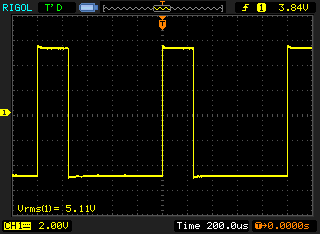
\includegraphics[width=0.46\textwidth]{pictures/NewFile7.png}
    \caption{Oscilograma temporal del tren de pulsos rectangulares ($T = \qty{1}{\milli\second}$, $t_0 = \qty{250}{\micro\second}$, $V_{\text{rms}} = \qty{5.11}{\volt}$).}
    \label{fig.ej2:tiempo_pulsos}
\end{figure}

\subsection{Comparación de Ventanas en el Tren de Pulsos}
Al acceder al \texttt{Math Menú} (FFT, CH1, Zoom X1 $\to$ Zoom X10, Promedio de 64 cuentas), se evaluó la variación de la
presentación al alternar entre ventanas:
\begin{itemize}
    \item Con ventana Rectangular (Figura~\ref{fig.ej2:rect}) se apreció una delimitación aguda de armónicos pero con
    lóbulos secundarios que elevaron la base.
    \item Con ventana Hanning (Figura~\ref{fig.ej2:hann}) se mitigó la fuga lateral.
    \item Dado que el osciloscopio Rigol DS1052E no dispone de ventana Flattop, se empleó en su lugar la ventana Blackman de acuerdo con las anotaciones de la consigna (\emph{«Usamos blacman»}), logrando una fuerte atenuación de los lóbulos de fuga y permitiendo visualizar con total nitidez los valles de la envolvente espectral.
\end{itemize}

\begin{figure}[!ht]
    \centering
    \begin{subfigure}[t]{0.48\textwidth}
        \centering
        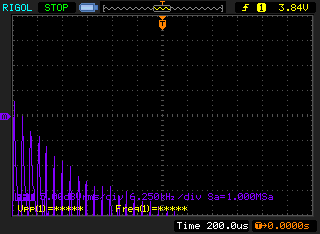
\includegraphics[width=\textwidth]{pictures/NewFile1.png}
        \caption{Ventana Rectangular.}
        \label{fig.ej2:rect}
    \end{subfigure}
    \hfill
    \begin{subfigure}[t]{0.48\textwidth}
        \centering
        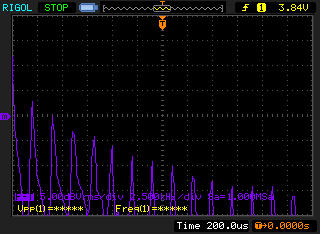
\includegraphics[width=\textwidth]{pictures/NewFile2.png}
        \caption{Ventana Hanning.}
        \label{fig.ej2:hann}
    \end{subfigure}
    \caption{Espectro del tren de pulsos según la ventana matemática seleccionada.}
    \label{fig.ej2:ventanas_pulsos}
\end{figure}

\subsection{Medición de Armónicos y Determinación del Período}
Configurando el osciloscopio en modo Promedio (64 cuentas) y ventana Rectangular, se ubicó el Cursor~1 en la componente
de continua ($f_0 = \qty{0.000}{\hertz}$) y con el Cursor~2 se midieron las frecuencias sucesivas $f_n$, calculando las
diferencias $\Delta f_n$ (Figura~\ref{fig.ej2:cursores_armonicos}). Los registros se exponen en el
Cuadro~\ref{tab.ej2:armonicos}.

\begin{figure}[!ht]
    \centering
    \begin{subfigure}[t]{0.48\textwidth}
        \centering
        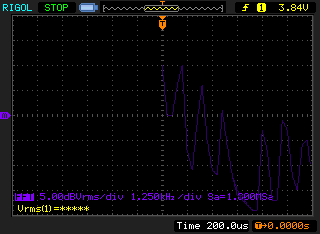
\includegraphics[width=\textwidth]{pictures/NewFile8.png}
        \caption{Medición de armónicos con cursores.}
        \label{fig.ej2:cursores_armonicos}
    \end{subfigure}
    \hfill
    \begin{subfigure}[t]{0.48\textwidth}
        \centering
        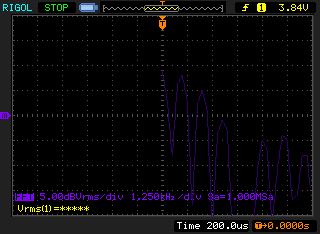
\includegraphics[width=\textwidth]{pictures/NewFile9.png}
        \caption{Identificación de valles espectrales.}
        \label{fig.ej2:cursores_valles}
    \end{subfigure}
    \caption{Medición de armónicos y valles espectrales mediante cursores de frecuencia.}
    \label{fig.ej2:mediciones_cursores}
\end{figure}

\begin{table}[!ht]
    \centering
    \resizebox{\textwidth}{!}{%
    \begin{tabular}{lccccc}
        \toprule
        \textbf{Cursor 2} & $f_1 = \qty{1}{\kilo\hertz}$ & $f_2 = \qty{2}{\kilo\hertz}$ & $f_3 = \qty{3}{\kilo\hertz}$ & $f_4 = \qty{5}{\kilo\hertz}$ & $f_5 = \qty{6}{\kilo\hertz}$ \\
        \midrule
        \textbf{$\Delta f_n$} & $\Delta f_{n1} = f_1 - f_0$ & $\Delta f_{n2} = f_2 - f_1$ & $\Delta f_{n3} = f_3 - f_2$ & $\Delta f_{n4} = f_4 - f_3$ & $\Delta f_{n5} = f_5 - f_4$ \\
        Diferencia med. & $\qty{1}{\kilo\hertz}$ & $\qty{1}{\kilo\hertz}$ & $\qty{1}{\kilo\hertz}$ & $\qty{2}{\kilo\hertz}$ & $\qty{1}{\kilo\hertz}$ \\
        \midrule
        \multicolumn{6}{c}{\textbf{$\Delta f_n\text{(promedio)}$:} $\qty{1.2}{\kilo\hertz}$ \quad $\implies$ \quad $T = 1 / \Delta f_n\text{(promedio)} = \qty{0.83}{\milli\second}$} \\
        \bottomrule
    \end{tabular}}
    \caption{Medición de componentes armónicas e intervalo entre rayas para el tren de pulsos.}
    \label{tab.ej2:armonicos}
\end{table}

\subsection{Medición de Valles y Determinación del Ancho de Pulso}
Cambiando a ventana Blackman (en reemplazo de Flattop no disponible), con el Cursor~2 se midieron las frecuencias correspondientes a los valles
(mínimos) de la gráfica (Figura~\ref{fig.ej2:cursores_valles}), volcados en el Cuadro~\ref{tab.ej2:valles}.

\begin{table}[!ht]
    \centering
    \begin{tabular}{lccc}
        \toprule
        \textbf{Cursor 2} & $f_a = \qty{4}{\kilo\hertz}$ & $f_b = \qty{8}{\kilo\hertz}$ & $f_c = \qty{12}{\kilo\hertz}$ \\
        \midrule
        \textbf{$\Delta f_{\text{min}}$} & $f_a - f_0 = \qty{4}{\kilo\hertz}$ & $f_b - f_a = \qty{4}{\kilo\hertz}$ & $f_c - f_b = \qty{4}{\kilo\hertz}$ \\
        \midrule
        \multicolumn{4}{c}{\textbf{$\Delta f_{\text{min}}\text{(promedio)}$:} $\qty{4}{\kilo\hertz}$ \quad $\implies$ \quad $t_0 = 1 / \Delta f_{\text{min}}\text{(promedio)} = \qty{0.25}{\milli\second} = \qty{250}{\micro\second}$} \\
        \bottomrule
    \end{tabular}
    \caption{Frecuencias de valles espectrales y cálculo del ancho de pulso ($t_0$).}
    \label{tab.ej2:valles}
\end{table}

El ancho de pulso deducido a partir de los valles del espectro ($t_0 = \qty{250}{\micro\second}$) coincide exactamente con
el valor fijado en el generador.

\subsection{Medición de la Componente de Continua}
Se seleccionó Amplitud en el menú Cursores para medir el pico correspondiente a $f_0 = \qty{0.000}{\hertz}$ en la FFT,
registrando un nivel de $\qty{8.0}{\dBV}$ (Figura~\ref{fig.ej2:medicion_cc}), cuya conversión a voltios es:
\begin{equation}
    V_{\text{CC(FFT)}} = 10^{\frac{8{,}0}{20}} = \qty{2.51}{\volt}
\end{equation}
Seguidamente, se midió la componente de continua en los bornes del generador con el multímetro digital en función $V_{\text{DC}}$:
\begin{equation}
    V_{\text{CC(Multímetro)}} = \qty{2.50}{\volt}
\end{equation}
Ambas lecturas concuerdan con el valor medio teórico del pulso ($V_{\text{med}} = D \cdot V_{\text{pico}} = 0{,}25 \cdot \qty{10}{\volt} = \qty{2.5}{\volt}$).

\begin{figure}[!ht]
    \centering
    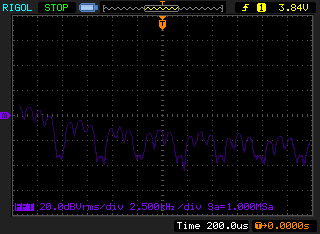
\includegraphics[width=0.46\textwidth]{pictures/NewFile11.png}
    \caption{Medición espectral de la componente de continua ($\qty{8.0}{\dBV_{\text{rms}}} \approx \qty{2.5}{\volt}$) en el dominio frecuencial.}
    \label{fig.ej2:medicion_cc}
\end{figure}

% =========================================================================
% EXPERIMENTO 3
% =========================================================================
\section{Experimento 3: Observación de Frecuencias \enquote{Alias}}
\label{sec.ej3:aliasing}

\subsection{Procedimiento y Circuito de Ensayo}
Se conectó el generador de funciones produciendo una onda senoidal de $\qty{10}{\kilo\hertz}$ a la entrada del osciloscopio
digital según el circuito de la Figura~\ref{crkt.ej3:medicion_alias}. En el \texttt{Math Menú} se configuró: FFT, CH1,
ventana Hanning y Zoom X1. A continuación, con la perilla \texttt{Sec/div} se ajustó la base de tiempos hasta fijar la
frecuencia de muestreo en:
\begin{equation}
    f_s = \qty{25.0}{\kilo\text{Sa\per\second}} \implies f_{\text{Nyq}} = \frac{f_s}{2} = \qty{12.5}{\kilo\hertz}
    \label{eq.ej3:nyquist}
\end{equation}

\begin{figure}[!ht]
    \centering
    % Circuito de medición para el Experimento 3: Observación de frecuencias Alias
\begin{circuitikz}[scale=0.9, transform shape]
    % Generador de funciones
    \draw (0,0) node[ground] {}
        to[sV, l={$G_1$ (\qty{10}{\kilo\hertz} a \qty{15.2}{\kilo\hertz})}] (0,2)
        to[short] (1.8,2);
    \draw (0,0) to[short] (1.8,0);

    % Conexión directa / Sonda al DSO (líneas horizontales paralelas)
    \draw (1.8,2) to[short, -o] (4.8,2) node[above, font=\scriptsize\bfseries] {CH1};
    \draw (1.8,0) to[short, -o] (4.8,0) node[above, font=\scriptsize\bfseries] {Masa};

    % Conexiones al panel del instrumento
    \draw (4.8,2) to[short] (5.4,2);
    \draw (4.8,0) to[short] (5.4,0);
    \draw (4.8,0) node[ground] {};

    % Bloque osciloscopio digital configurado para submuestreo
    \draw[thick, rounded corners=3pt, fill=blue!3] (5.4,-0.8) rectangle (10.2,2.8);
    \node at (7.8,2.2) [font=\bfseries\small] {Osciloscopio DSO};
    \node at (7.8,1.5) [font=\scriptsize, align=center] {Base de tiempos: SEC/DIV ajustado\\Frec. Muestreo: $f_s = \qty{25.0}{\kilo\Sa\per\second}$};
    \node at (7.8,0.7) [font=\scriptsize, align=center] {Límite Nyquist: $f_{\text{Nyq}} = \qty{12.5}{\kilo\hertz}$};
    \node at (7.8,-0.1) [font=\tiny, align=center] {Modo FFT / Ventana Hanning};
\end{circuitikz}

    \caption{Circuito de conexión para la observación experimental del fenómeno de Alias.}
    \label{crkt.ej3:medicion_alias}
\end{figure}

Se verificó mediante el menú Cursores que la frecuencia inicial de la señal fuera efectivamente $\qty{10}{\kilo\hertz}$
(Figura~\ref{fig.ej3:alias10k}).

\begin{figure}[!ht]
    \centering
    \begin{subfigure}[t]{0.48\textwidth}
        \centering
        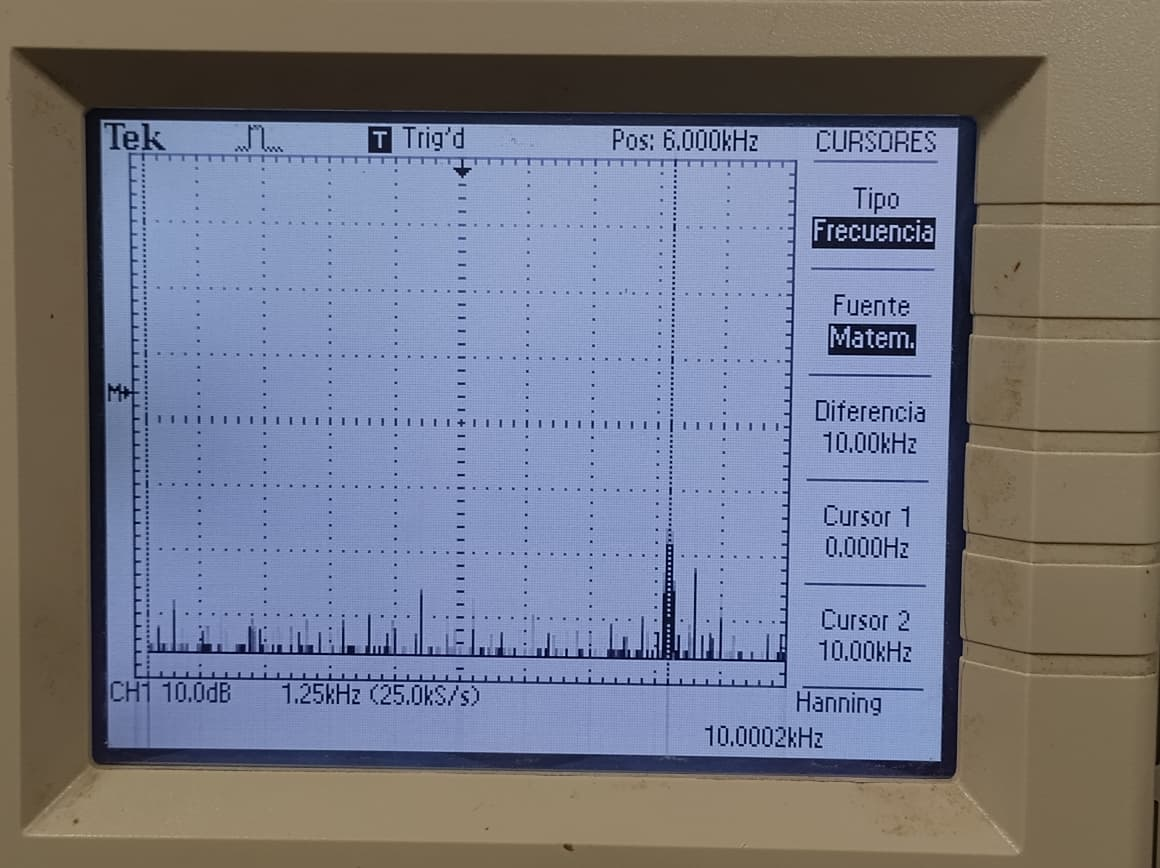
\includegraphics[width=\textwidth]{pictures/foto1.jpg}
        \caption{Señal a $\qty{10.00}{\kilo\hertz}$ ($f_{\text{in}} < f_{\text{Nyq}}$).}
        \label{fig.ej3:alias10k}
    \end{subfigure}
    \hfill
    \begin{subfigure}[t]{0.48\textwidth}
        \centering
        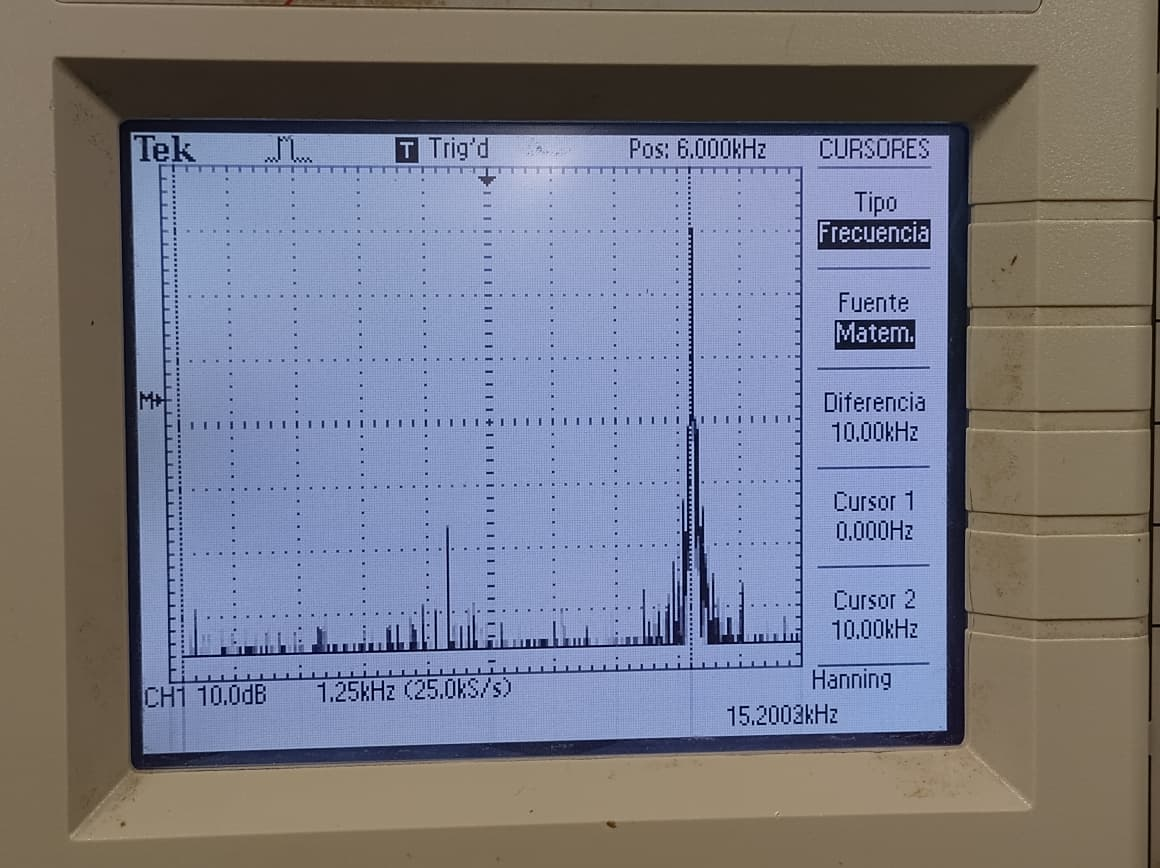
\includegraphics[width=\textwidth]{pictures/foto2.jpg}
        \caption{Repliegue a $\qty{9.8}{\kilo\hertz}$ ($f_{\text{in}} = \qty{15.2}{\kilo\hertz}$).}
        \label{fig.ej3:alias15k}
    \end{subfigure}
    \caption{Observación experimental del repliegue espectral en la frecuencia de Nyquist ($\qty{12.5}{\kilo\hertz}$).}
    \label{fig.ej3:aliasing_senoidal}
\end{figure}

\subsection{Observación del Repliegue en Nyquist}
Manteniendo el cursor de referencia fijo en $\qty{10}{\kilo\hertz}$, se incrementó progresivamente la frecuencia del
generador. Al sobrepasar la frecuencia de Nyquist ($\qty{12.5}{\kilo\hertz}$), la raya espectral comenzó a retroceder
hacia la izquierda (repliegue). Al situar la señal en $f_{\text{in}} = \qty{15.20}{\kilo\hertz}$, en la pantalla apareció
una componente aparente (falsa) en:
\begin{equation}
    f_{\text{alias}} = |f_s - f_{\text{in}}| = |\qty{25.0}{\kilo\hertz} - \qty{15.20}{\kilo\hertz}| = \qty{9.80}{\kilo\hertz}
\end{equation}
tal como se constata en el oscilograma de la Figura~\ref{fig.ej3:alias15k} (en las anotaciones de la guía:
\emph{\enquote{el pico sale fuera y se repliega}}).

\subsection{Ensayo con Forma de Onda Cuadrada}
Se conmutó la salida del generador a onda cuadrada. Al contener infinitos armónicos impares, todos aquellos armónicos
que superaron los $\qty{12.5}{\kilo\hertz}$ se replegaron sobre la banda base, generando un conjunto de rayas espurias
que contaminaron severamente el espectro (Figura~\ref{fig.ej3:aliasing_cuadrada}).

\begin{figure}[!ht]
    \centering
    \begin{subfigure}[t]{0.31\textwidth}
        \centering
        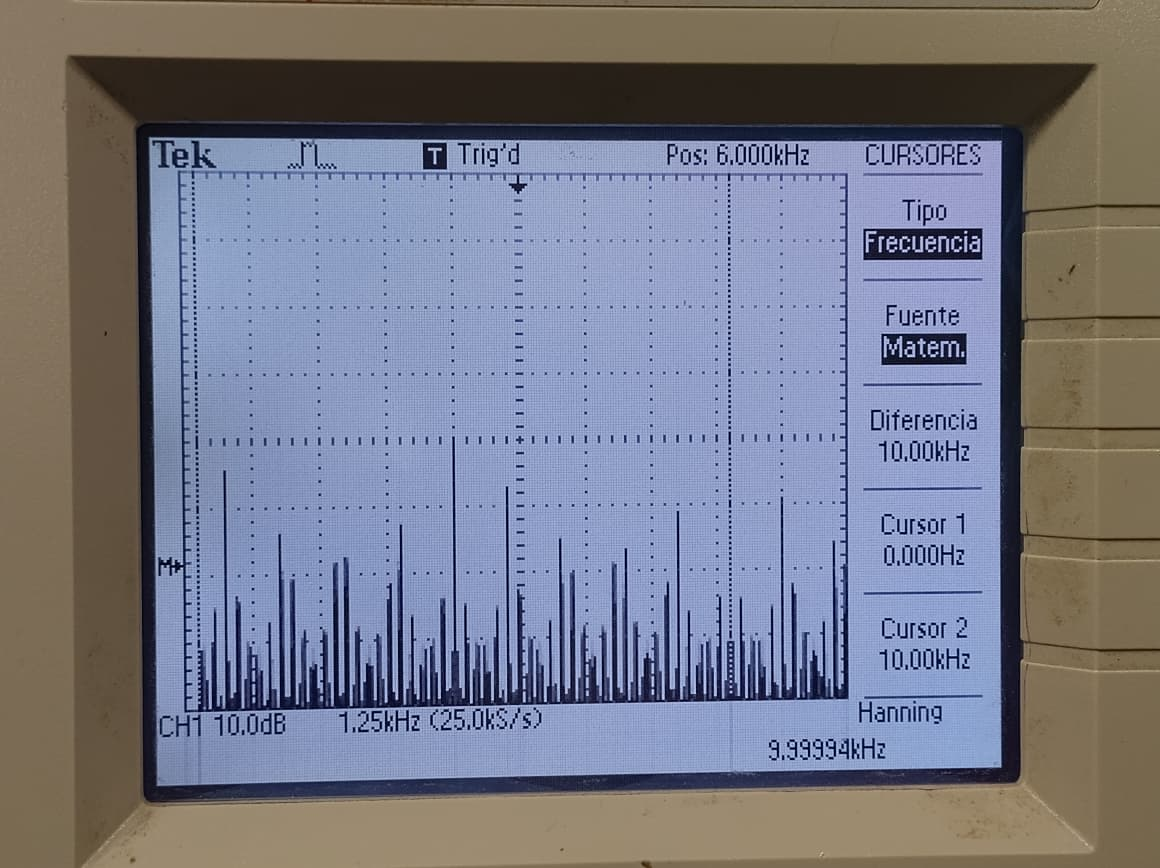
\includegraphics[width=\textwidth]{pictures/foto3.jpg}
        \caption{Cuadrada en $\qty{10}{\kilo\hertz}$.}
        \label{fig.ej3:cuadrada10k}
    \end{subfigure}
    \hfill
    \begin{subfigure}[t]{0.31\textwidth}
        \centering
        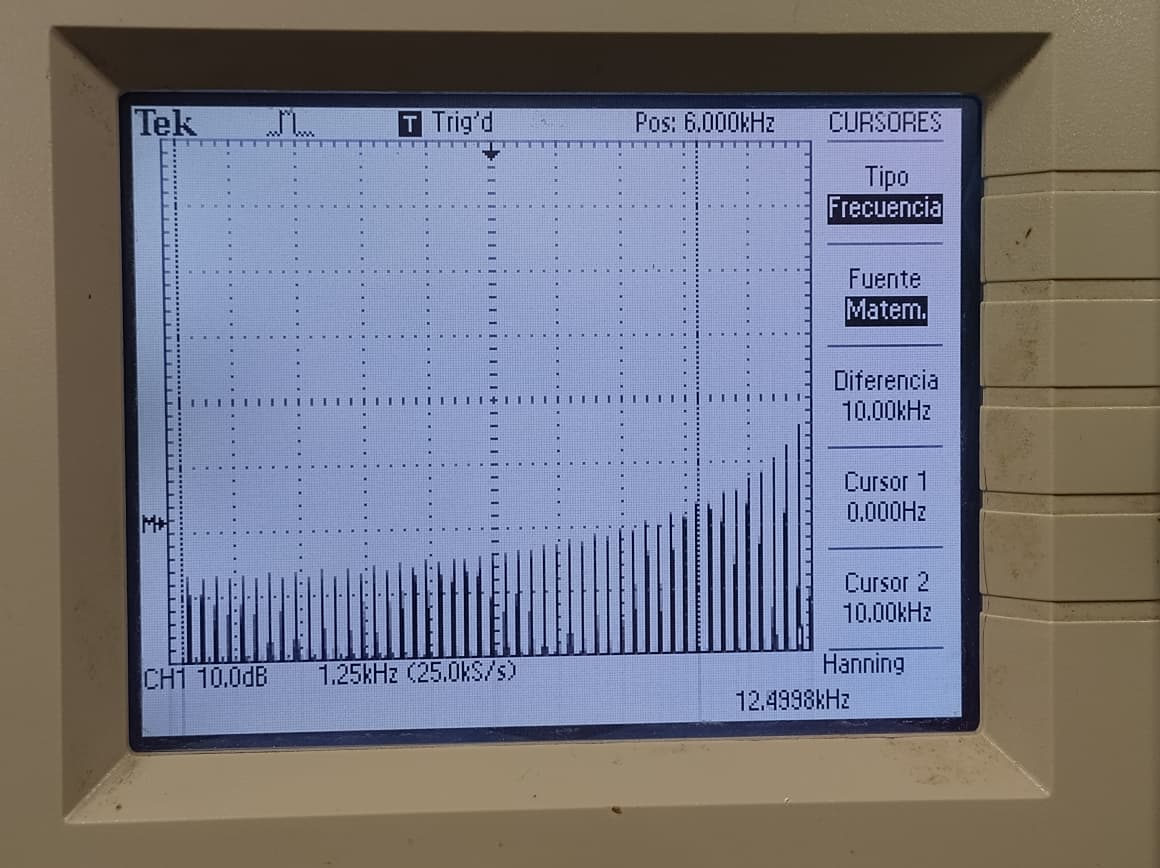
\includegraphics[width=\textwidth]{pictures/foto4.jpg}
        \caption{Cuadrada en $\qty{12.5}{\kilo\hertz}$.}
        \label{fig.ej3:cuadradanyq}
    \end{subfigure}
    \hfill
    \begin{subfigure}[t]{0.31\textwidth}
        \centering
        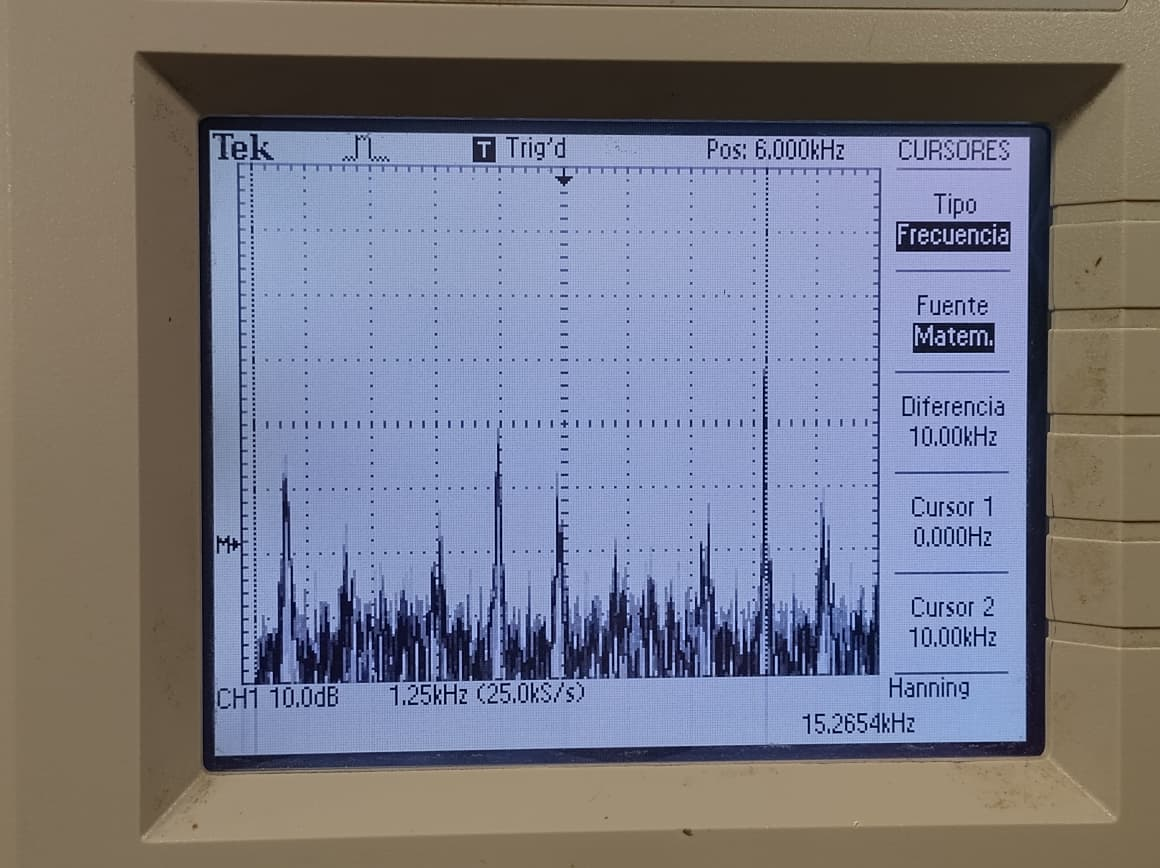
\includegraphics[width=\textwidth]{pictures/foto5.jpg}
        \caption{Cuadrada en $\qty{15.26}{\kilo\hertz}$.}
        \label{fig.ej3:cuadrada15k}
    \end{subfigure}
    \caption{Contaminación por armónicos replegados al muestrear onda cuadrada con velocidad insuficiente.}
    \label{fig.ej3:aliasing_cuadrada}
\end{figure}

% =========================================================================
% EXPERIMENTO 4
% =========================================================================
\section{Experimento 4: Análisis de una Señal Modulada en Amplitud}
\label{sec.ej4:modulacion_am}

\subsection{Procedimiento y Circuito Modulador}
Para generar la señal de amplitud modulada se implementó el circuito modulador sencillo especificado en la
Figura~1 de la consigna, cuyo esquema eléctrico se detalla en la Figura~\ref{crkt.ej4:modulador_am} y cuya placa
experimental de laboratorio se muestra en la Figura~\ref{fig.ej4:foto_modulador}.

\begin{figure}[!ht]
    \centering
    % Circuito esquemático del modulador de amplitud (Figura 1 de la consigna)
\begin{circuitikz}[scale=0.82, transform shape]
    % Generador 1 (Portadora 50 kHz)
    \draw (0,1.8) node[ground] {}
        to[sV, l={$G_1\ (f_c \approx \qty{50}{\kilo\hertz})$}] (0,3.6)
        to[R, l={$R_1 = 4{,}7\,\unit{k\Omega}$}] (3.5,3.6)
        -- (3.5,1.8);

    % Generador 2 (Modulante 1 kHz)
    \draw (0,-1.8) node[ground] {}
        to[sV, l={$G_2\ (f_m = \qty{1}{\kilo\hertz})$}] (0,0)
        to[R, l={$R_2 = 4{,}7\,\unit{k\Omega}$}] (3.5,0)
        -- (3.5,1.8);

    % Nodo sumador y Diodo mezclador
    \draw (3.5,1.8) to[short, *-] (4.0,1.8)
        to[D, l={$D_1$ (RF)}, -*] (5.8,1.8);

    % Circuito tanque LC sintonizado en paralelo a masa
    % Rama capacitor (etiqueta a la izquierda con l_)
    \draw (5.8,1.8) -- (6.6,1.8)
        to[C, l_={$C = 10\,\unit{nF}$}, *-*] (6.6,-0.6);
    
    % Rama inductor con separación generosa de 2.2 cm (etiqueta a la derecha con l)
    \draw (6.6,1.8) -- (8.8,1.8)
        to[L, l={$L = 1\,\unit{mH}$}, *-*] (8.8,-0.6);
    
    % Unión inferior a masa
    \draw (6.6,-0.6) -- (8.8,-0.6) node[midway, ground] {};

    % Conexión de salida al Osciloscopio con FFT
    \draw (8.8,1.8) to[short, -*] (9.6,1.8)
        to[short, -o] (10.4,1.8) node[above, font=\scriptsize] {Salida (A.M) $\to$ DSO};
\end{circuitikz}

    \caption{Esquema eléctrico del modulador de amplitud (Figura 1 de la consigna).}
    \label{crkt.ej4:modulador_am}
\end{figure}

\begin{figure}[!ht]
    \centering
    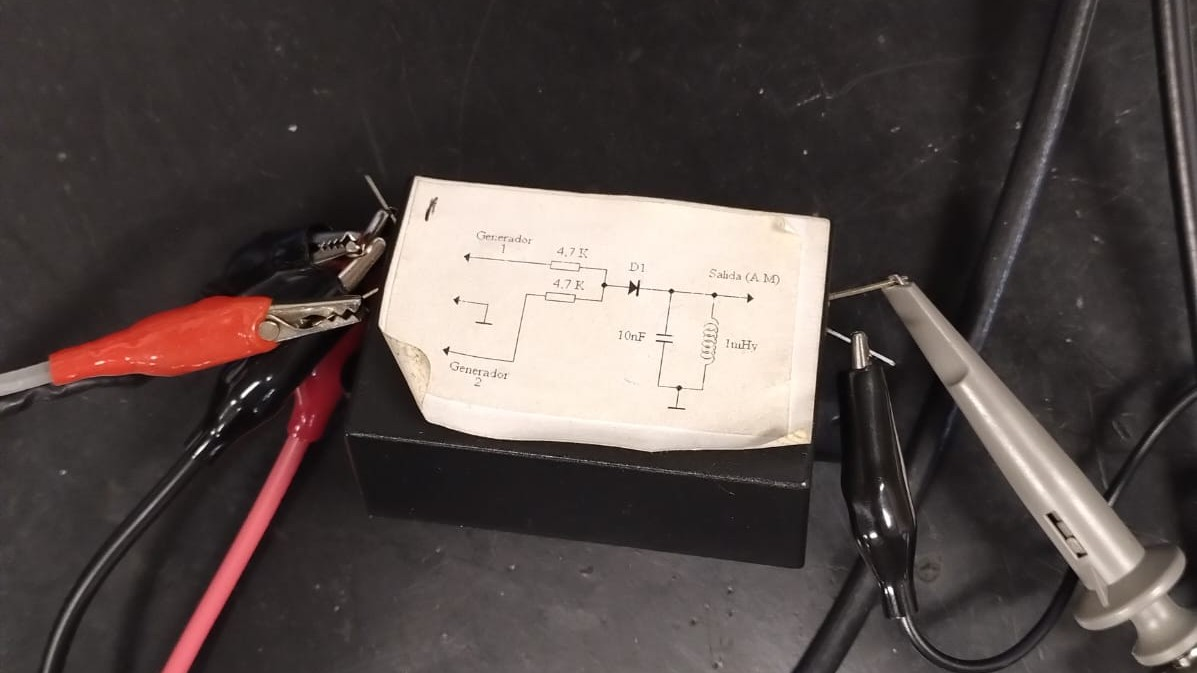
\includegraphics[width=0.45\textwidth]{pictures/foto11.jpg}
    \caption{Módulo físico del circuito modulador de amplitud empleado en el laboratorio.}
    \label{fig.ej4:foto_modulador}
\end{figure}

El circuito emplea un diodo de señal para RF ($D_1$) como elemento no lineal sumador y un circuito tanque paralelo
($C = \qty{10}{\nano\farad}$, $L = \qty{1}{\milli\henry}$) sintonizado para resonar en aproximadamente $\qty{50}{\kilo\hertz}$.
Se dispusieron dos generadores:
\begin{itemize}
    \item Generador 1 ($G_1$): Portadora senoidal de $f_c = \qty{50}{\kilo\hertz}$, nivel en media vuelta.
    \item Generador 2 ($G_2$): Modulante senoidal de $f_m = \qty{1}{\kilo\hertz}$, nivel en un cuarto de vuelta.
\end{itemize}

En el osciloscopio se ajustó la base de tiempos con la perilla \texttt{Sec/div} en $\qty{1}{\milli\second\per\text{div}}$
para observar la envolvente de modulación sobre la portadora (Figura~\ref{fig.ej4:tiempo_am}). Se estabilizó el disparo
mediante el menú \texttt{Trigger} (Pendiente: +, Fuente: CH1, Modo: Auto, Acoplamiento: Rechazo AF). Luego se accedió al
\texttt{Math Menú} configurando FFT en CH1, ventana Hanning, Zoom X10 y Promedio de 64 cuentas (Figura~\ref{fig.ej4:espectro_am}).

\begin{figure}[!ht]
    \centering
    \begin{subfigure}[t]{0.48\textwidth}
        \centering
        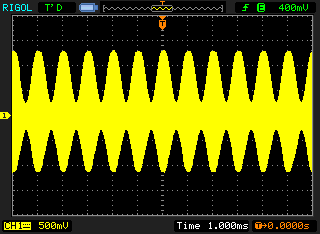
\includegraphics[width=\textwidth]{pictures/NewFile12.png}
        \caption{Envolvente temporal ($\qty{1}{\milli\second\per\text{div}}$).}
        \label{fig.ej4:tiempo_am}
    \end{subfigure}
    \hfill
    \begin{subfigure}[t]{0.48\textwidth}
        \centering
        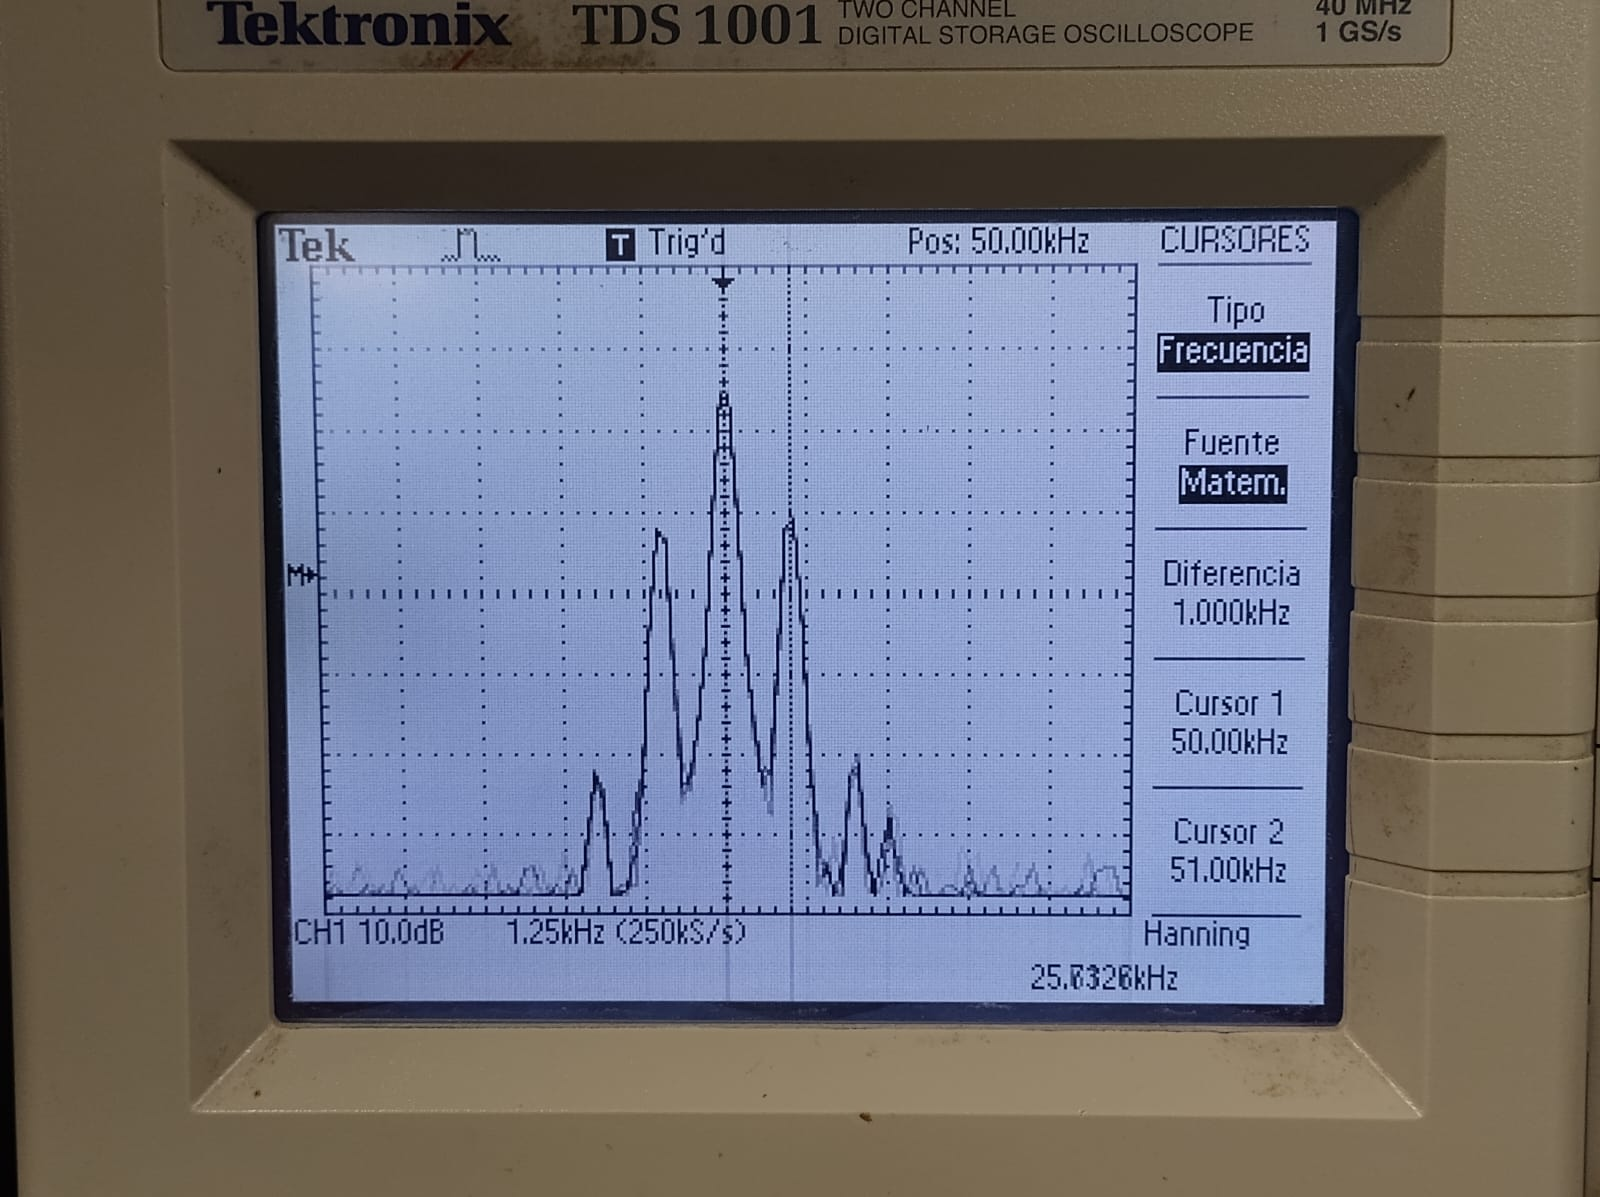
\includegraphics[width=\textwidth]{pictures/foto8.jpg}
        \caption{Espectro FFT con ventana Hanning.}
        \label{fig.ej4:espectro_am}
    \end{subfigure}
    \caption{Visualización temporal y espectral de la señal modulada en amplitud.}
    \label{fig.ej4:am_temporal_y_espectro}
\end{figure}

\subsection{Mediciones y Cálculo del Índice de Modulación}
Mediante el menú Cursores se efectuaron las mediciones de frecuencia y amplitud requeridas:
\begin{itemize}
    \item Frecuencia portadora (Port): $\qty{50}{\kilo\hertz}$.
    \item Frecuencia lateral sup/inf (FL\_): $\qty{49}{\kilo\hertz} \text{ / } \qty{51}{\kilo\hertz}$.
    \item Frecuencia modulante ($\text{Dif.} = \text{FLS} - f_c$): $\qty{1}{\kilo\hertz}$.
    \item Amplitud Portadora ($\text{dB}_{\text{portadora}}$): $\qty{-5}{\dBV}$.
    \item Amplitud Banda Lateral ($\text{dB}_{\text{B.lateral}}$): $\qty{-19.5}{\dBV}$.
\end{itemize}

Con estos valores se calculó el índice de modulación $m$ mediante las fórmulas consignadas:
\begin{equation}
    m_{(\text{dB})} = \text{dB}_{\text{B.lateral}} - \text{dB}_{\text{Portadora}} + \qty{6}{\decibel} =
    -19{,}5 - (-5) + 6 = \qty{-8.5}{\decibel}
    \label{eq.ej4:mdb}
\end{equation}
\begin{equation}
    m = 10^{\frac{m(\text{dB})}{20}} = 10^{\frac{-8{,}5}{20}} \approx 0{,}38
    \label{eq.ej4:mlineal}
\end{equation}

\subsection{Observaciones con Distintas Formas de Onda y Ventanas}
Siguiendo la guía:
\begin{itemize}
    \item Se conmutó la modulante a onda cuadrada (Figura~\ref{fig.ej4:am_cuadrada}) y triangular (Figura~\ref{fig.ej4:am_triangular}),
    observando la aparición de múltiples bandas laterales armónicas en el espectro.
    \item Se compararon las ventanas Flattop (Figura~\ref{fig.ej4:flattop_am}) y Rectangular (Figura~\ref{fig.ej4:rect_am}),
    comprobando que Flattop aplana la cima permitiendo una medición exacta de los decibeles, mientras que Rectangular
    presenta lóbulos de derrame en la base.
\end{itemize}

\begin{figure}[!ht]
    \centering
    \begin{subfigure}[t]{0.48\textwidth}
        \centering
        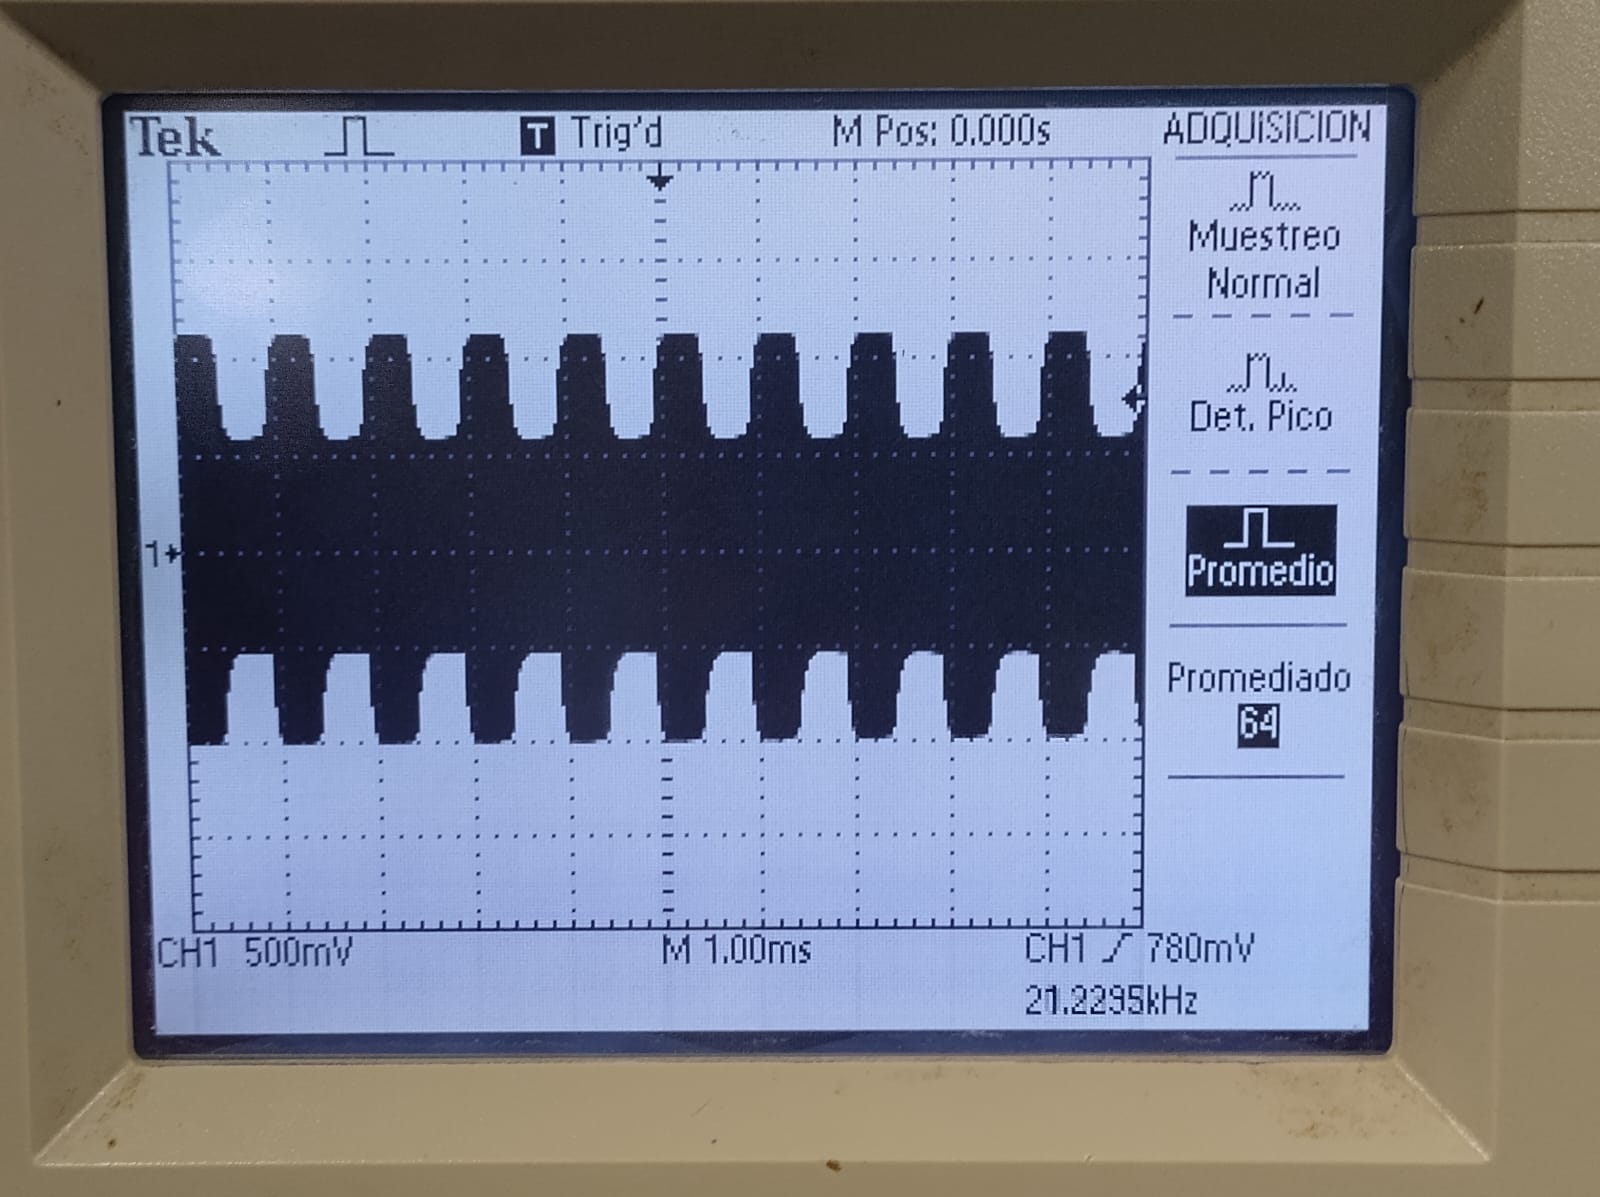
\includegraphics[width=\textwidth]{pictures/foto6.jpg}
        \caption{Modulante cuadrada.}
        \label{fig.ej4:am_cuadrada}
    \end{subfigure}
    \hfill
    \begin{subfigure}[t]{0.48\textwidth}
        \centering
        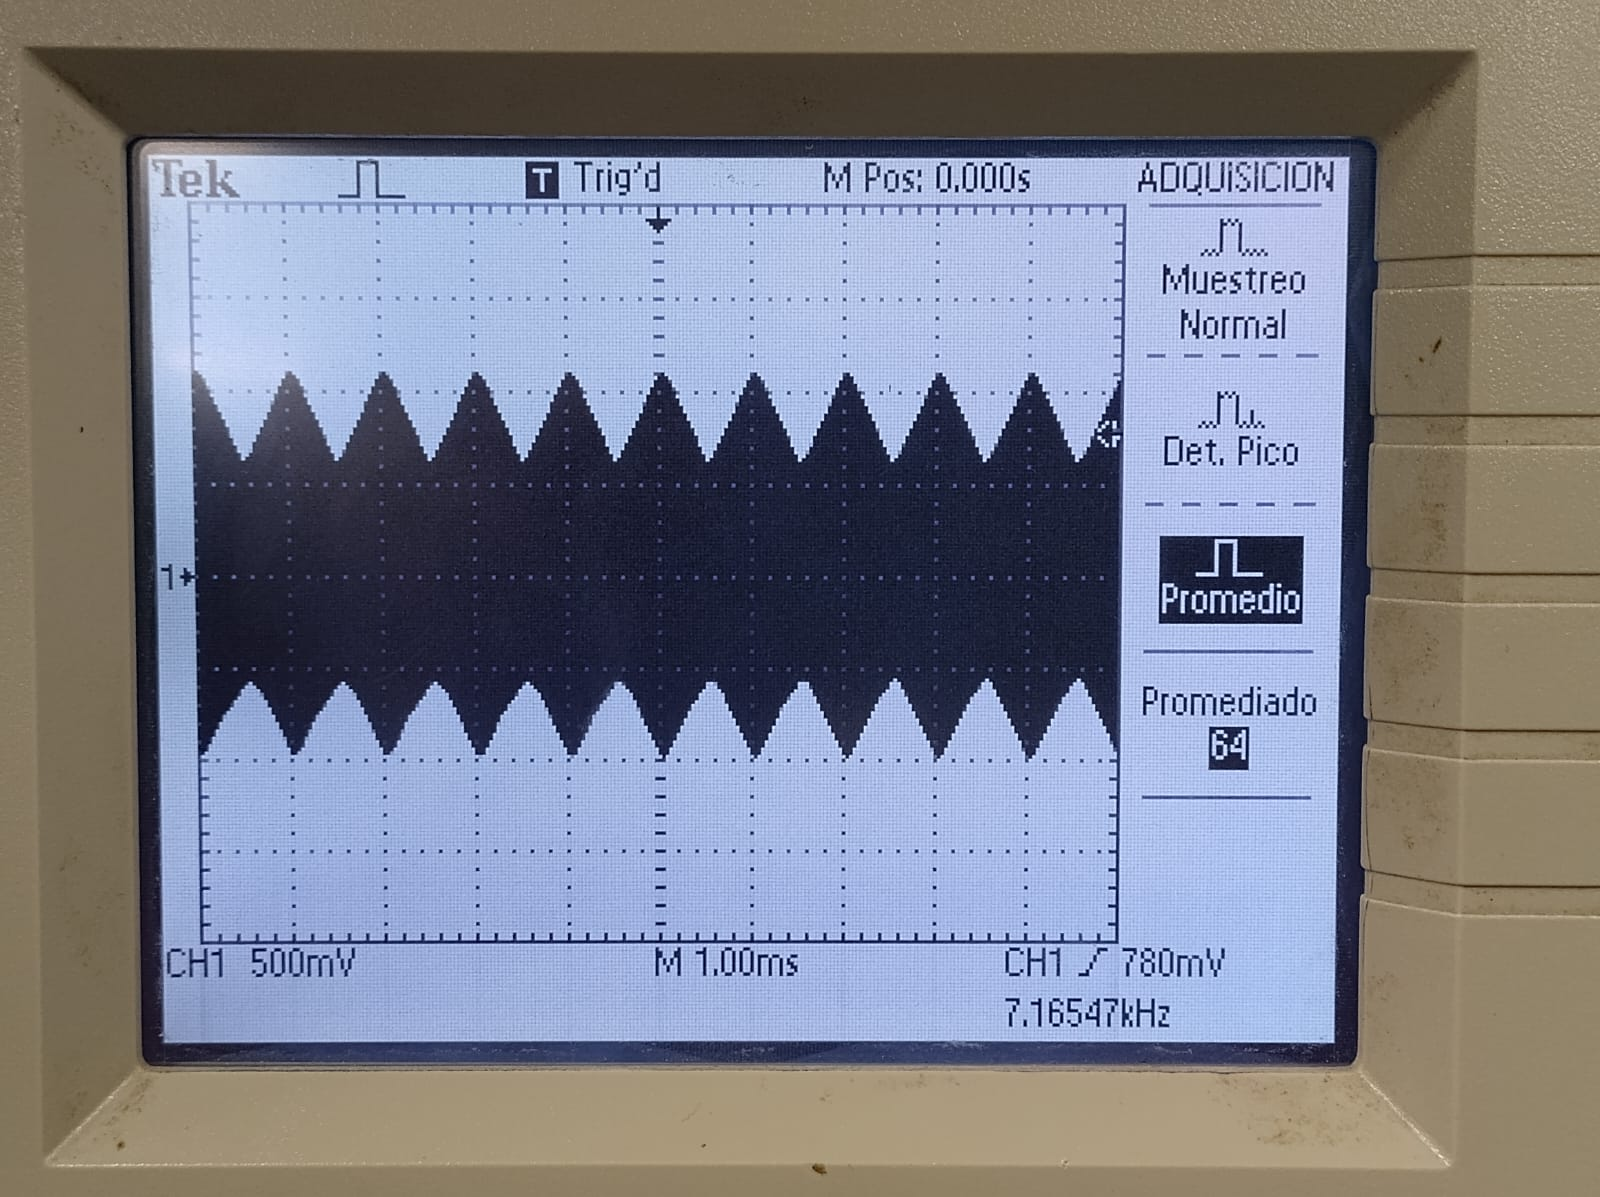
\includegraphics[width=\textwidth]{pictures/foto7.jpg}
        \caption{Modulante triangular.}
        \label{fig.ej4:am_triangular}
    \end{subfigure}
    \caption{Envolventes temporales de modulación en amplitud con modulantes compleja.}
    \label{fig.ej4:modulantes_am}
\end{figure}

\begin{figure}[!ht]
    \centering
    \begin{subfigure}[t]{0.48\textwidth}
        \centering
        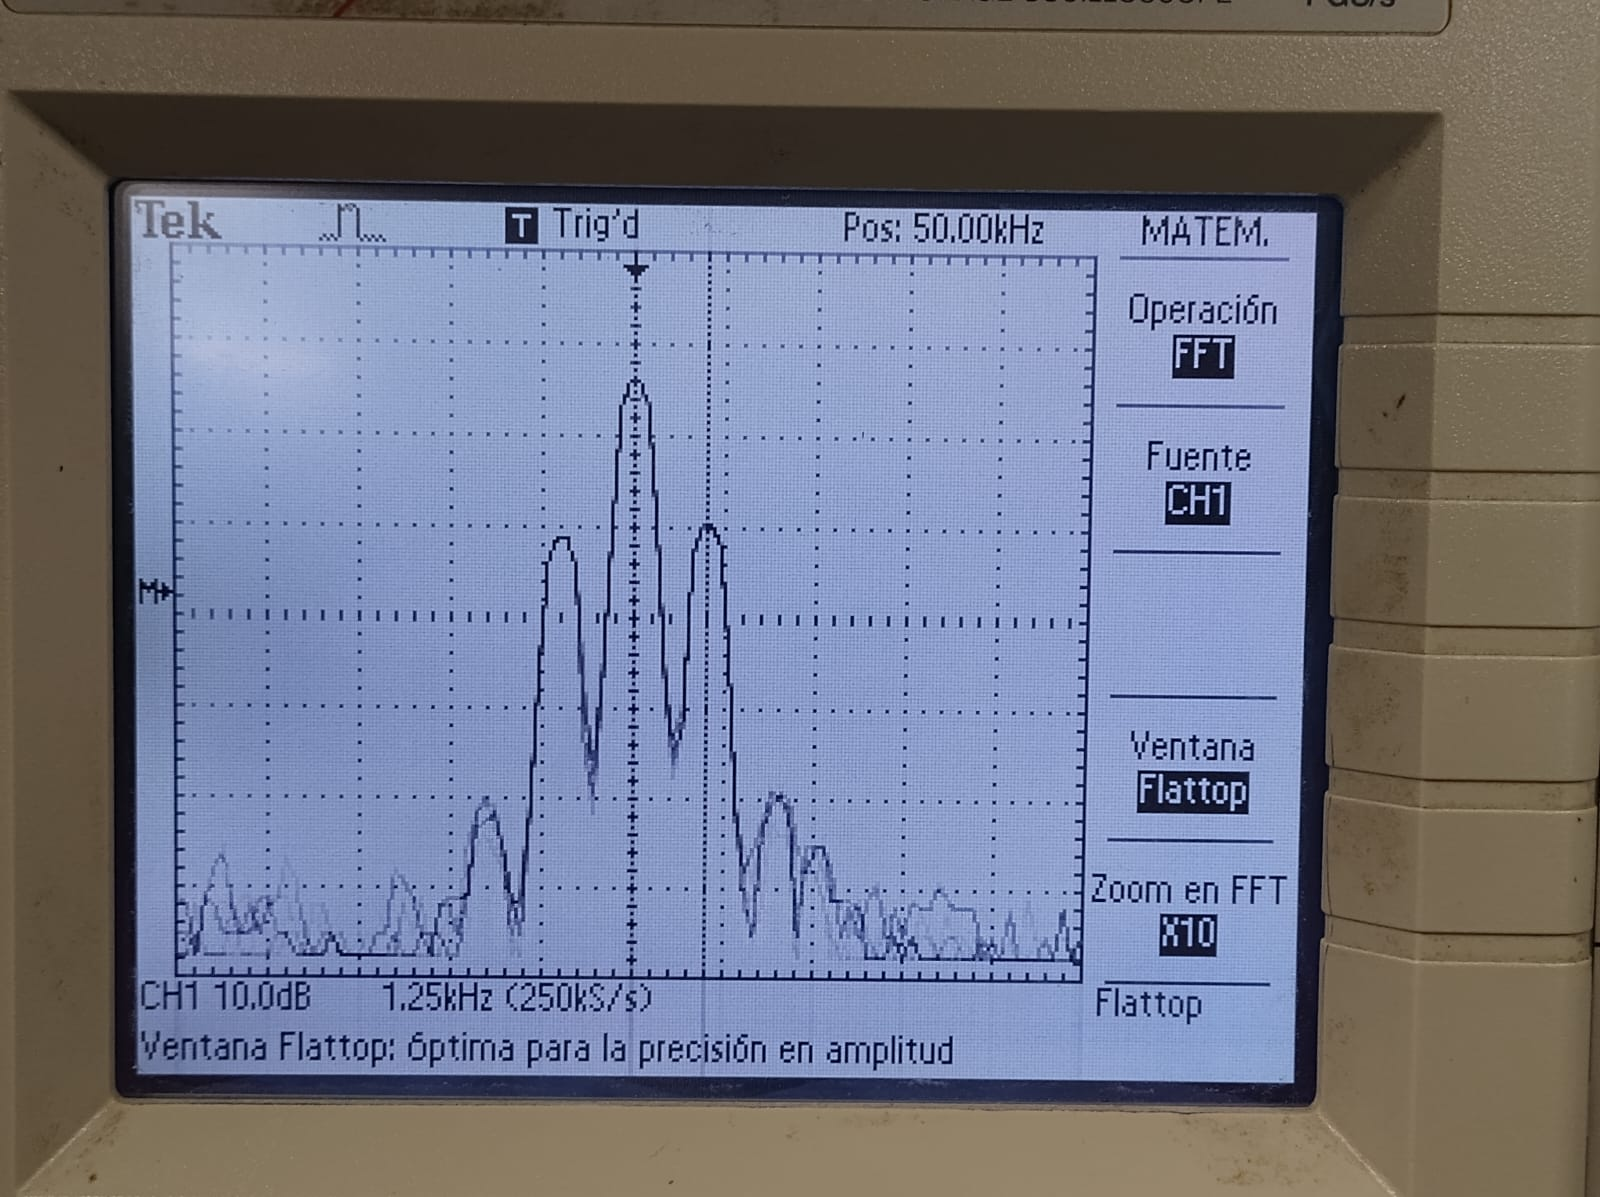
\includegraphics[width=\textwidth]{pictures/foto9.jpg}
        \caption{Ventana Flattop.}
        \label{fig.ej4:flattop_am}
    \end{subfigure}
    \hfill
    \begin{subfigure}[t]{0.48\textwidth}
        \centering
        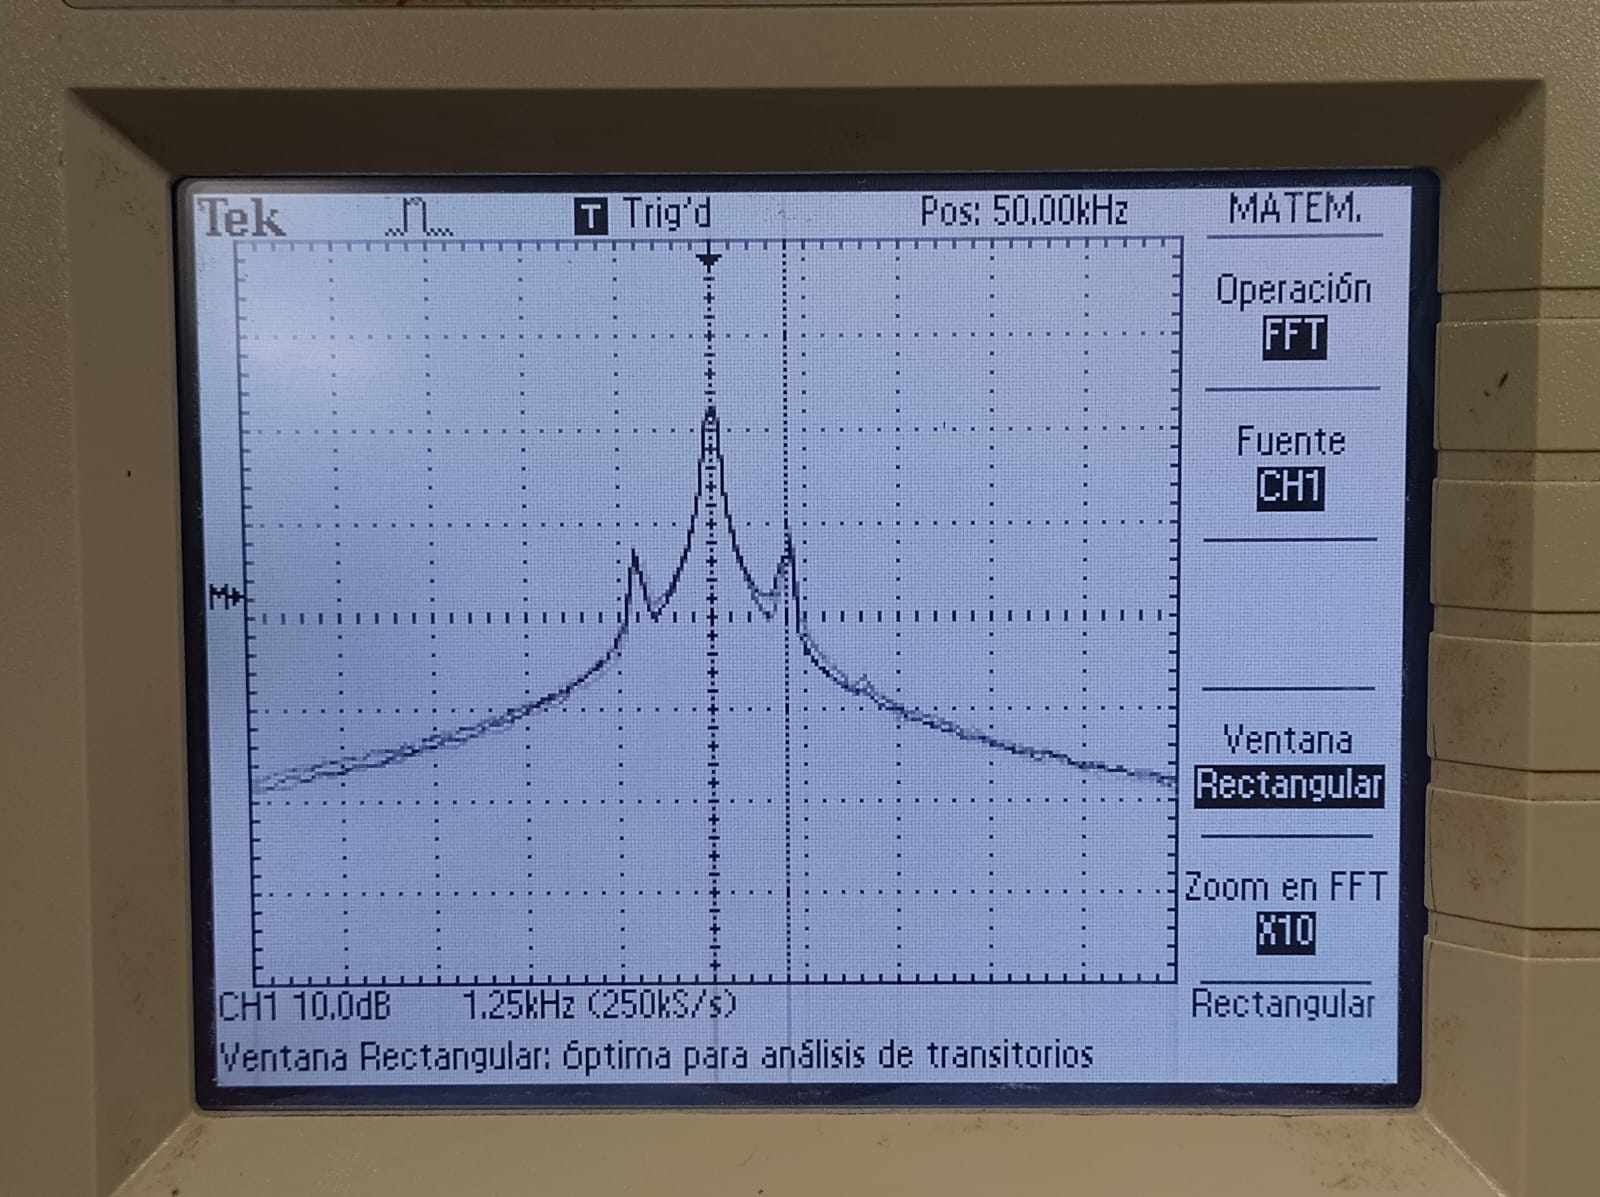
\includegraphics[width=\textwidth]{pictures/foto10.jpg}
        \caption{Ventana Rectangular.}
        \label{fig.ej4:rect_am}
    \end{subfigure}
    \caption{Comparación de ventanas matemáticas en el espectro de la señal AM.}
    \label{fig.ej4:ventanas_am}
\end{figure}

% =========================================================================
% EXPERIMENTO 5
% =========================================================================
\section{Experimento 5: Observación de los Productos de IMD de Tercer Orden}
\label{sec.ej5:intermodulacion}

\subsection{Procedimiento y Circuito de Medición}
El modulador a diodo aprovecha la no linealidad cuadrática para modular en amplitud; no obstante, las alinealidades de
orden superior dan lugar a los productos de intermodulación (IMD), siendo los más relevantes los de tercer orden.
Se utilizó el mismo circuito modulador pero excitado con dos generadores senoidales según la
Figura~\ref{crkt.ej5:medicion_imd}.

\begin{figure}[!ht]
    \centering
    % Circuito de medición para el Experimento 5: Ensayo de IMD de tercer orden
\begin{circuitikz}[scale=0.82, transform shape]
    % Generador 1 (Tono 1: 49 kHz)
    \draw (0,1.8) node[ground] {}
        to[sV, l={$G_1\ (\qty{49}{\kilo\hertz})$}] (0,3.6)
        to[R, l={$R_1 = 4{,}7\,\unit{k\Omega}$}] (3.5,3.6)
        -- (3.5,1.8);

    % Generador 2 (Tono 2: 51 kHz)
    \draw (0,-1.8) node[ground] {}
        to[sV, l={$G_2\ (\qty{51}{\kilo\hertz})$}] (0,0)
        to[R, l={$R_2 = 4{,}7\,\unit{k\Omega}$}] (3.5,0)
        -- (3.5,1.8);

    % Diodo y tanque LC
    \draw (3.5,1.8) to[short, *-] (4.0,1.8)
        to[D, l={$D_1$ (RF)}, -*] (5.6,1.8);

    \draw (5.6,1.8) -- (6.4,1.8)
        to[C, l_={$C = 10\,\unit{nF}$}, *-*] (6.4,-0.6);
    \draw (6.4,1.8) -- (8.4,1.8)
        to[L, l={$L = 1\,\unit{mH}$}, *-*] (8.4,-0.6);
    \draw (6.4,-0.6) -- (8.4,-0.6) node[midway, ground] {};

    % Conexión hacia el osciloscopio digital (líneas paralelas con etiquetas arriba)
    \draw (8.4,1.8) to[short, -o] (10.2,1.8) node[above, font=\scriptsize\bfseries] {CH1};
    \draw (8.4,-0.6) to[short, -o] (10.2,-0.6) node[above, font=\scriptsize\bfseries] {Masa};

    % Conexiones al panel del DSO
    \draw (10.2,1.8) to[short] (10.8,1.8);
    \draw (10.2,-0.6) to[short] (10.8,-0.6);
    \draw (10.2,-0.6) node[ground] {};

    % Bloque osciloscopio
    \draw[thick, rounded corners=3pt, fill=blue!3] (10.8,-1.0) rectangle (15.4,2.8);
    \node at (13.1,2.3) [font=\bfseries\small] {Osciloscopio DSO};
    \node at (13.1,1.55) [font=\scriptsize, align=center] {FFT / Ventana Hanning\\Zoom X10 / Cursores};
    \node at (13.1,0.7) [font=\scriptsize, align=center] {Medición de tonos $f_1, f_2$\\y productos IMD3};
    \node at (13.1,-0.2) [font=\tiny, align=center] {Rechazo $\Delta(\text{dB}) = \qty{35.2}{\decibel}$};
\end{circuitikz}

    \caption{Circuito de conexión para el ensayo de intermodulación de tercer orden con dos tonos.}
    \label{crkt.ej5:medicion_imd}
\end{figure}

Primero se encendió $G_1$ solo y se retocó su frecuencia hasta localizar el punto de máxima sintonía del circuito
resonante, registrándose en $f_{\text{res}} = \qty{51.5}{\kilo\hertz}$. Luego se apagó $G_1$ y se calibró $G_2$ para
obtener igual nivel. Finalmente, se encendieron ambos generadores retocando sus frecuencias para que quedaran
equidistantes del pico de sintonía con una separación de $\qty{2}{\kilo\hertz}$ ($f_1 = \qty{49}{\kilo\hertz}$,
$f_2 = \qty{51}{\kilo\hertz}$).

\subsection{Mediciones de IMD3 y Rechazo Obtenido}
En la Figura~\ref{fig.ej5:foto_imd} se presenta el oscilograma del espectro obtenido en el osciloscopio digital con ventana Hanning.

\begin{figure}[!ht]
    \centering
    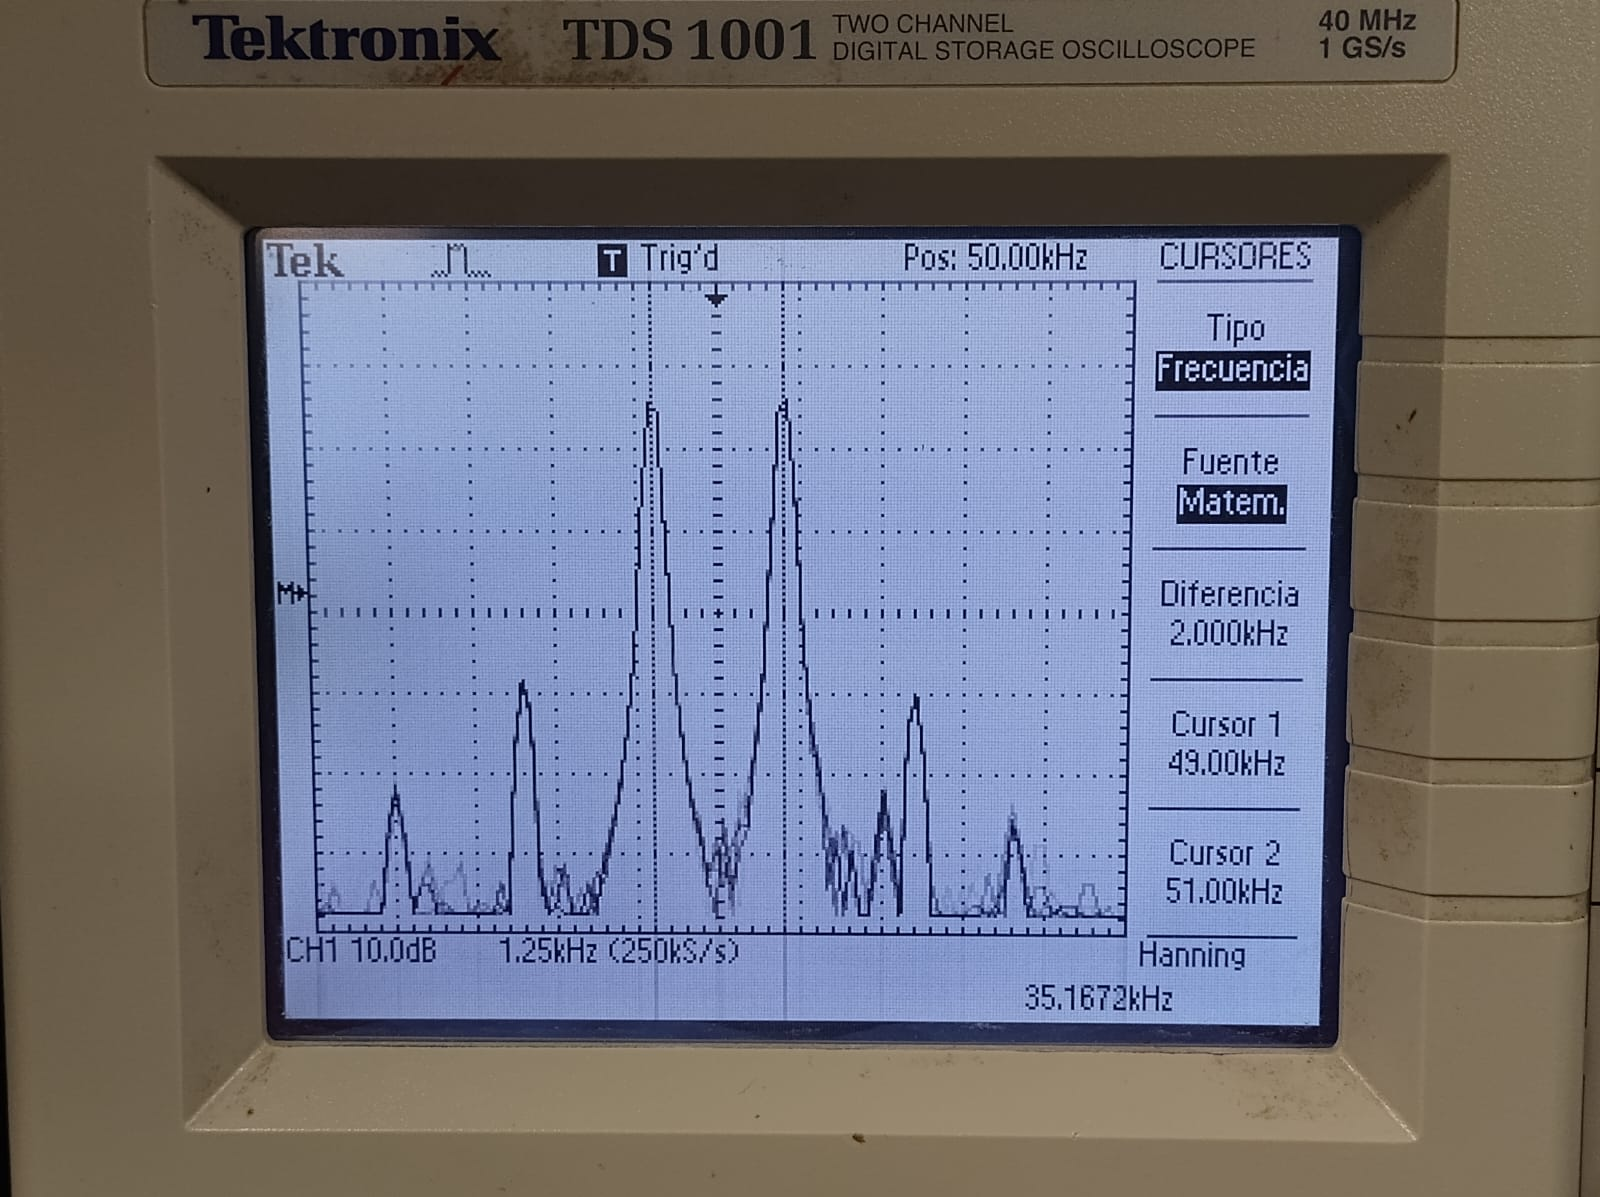
\includegraphics[width=0.46\textwidth]{pictures/foto12.jpg}
    \caption{Espectro FFT con los tonos fundamentales $f_1, f_2$ y los productos de IMD3 ($2f_1-f_2, 2f_2-f_1$).}
    \label{fig.ej5:foto_imd}
\end{figure}

Los valores registrados en la guía son:
\begin{itemize}
    \item $f_1 = \qty{49}{\kilo\hertz}$
    \item $f_2 = \qty{51}{\kilo\hertz}$
    \item $2f_1 - f_2 = 2(\qty{49}{\kilo\hertz}) - \qty{51}{\kilo\hertz} = \qty{47}{\kilo\hertz}$
    \item $2f_2 - f_1 = 2(\qty{51}{\kilo\hertz}) - \qty{49}{\kilo\hertz} = \qty{53}{\kilo\hertz}$
    \item \textbf{Rechazo de IMD de 3er orden [$\Delta(\text{dB})$]:} $\qty{35.2}{\decibel}$.
\end{itemize}

% =========================================================================
% EXPERIMENTO 6
% =========================================================================
\section{Experimento 6: Análisis de una Señal Modulada en Frecuencia}
\label{sec.ej6:modulacion_fm}

\subsection{Procedimiento y Diagrama de Conexión}
Aprovechando la entrada de control por tensión (VCF) del generador principal GW INSTEK GFG-3015, se conectó la salida
del segundo generador ($G_2$) a dicha entrada a través de un potenciómetro de $\qty{1}{\kilo\ohm}$ como atenuador,
configurando el conjunto como generador de FM según el diagrama de la Figura~\ref{crkt.ej6:conexion_fm}.

\begin{figure}[!ht]
    \centering
    % Diagrama de conexión para la generación y medición de señal FM mediante entrada VCF
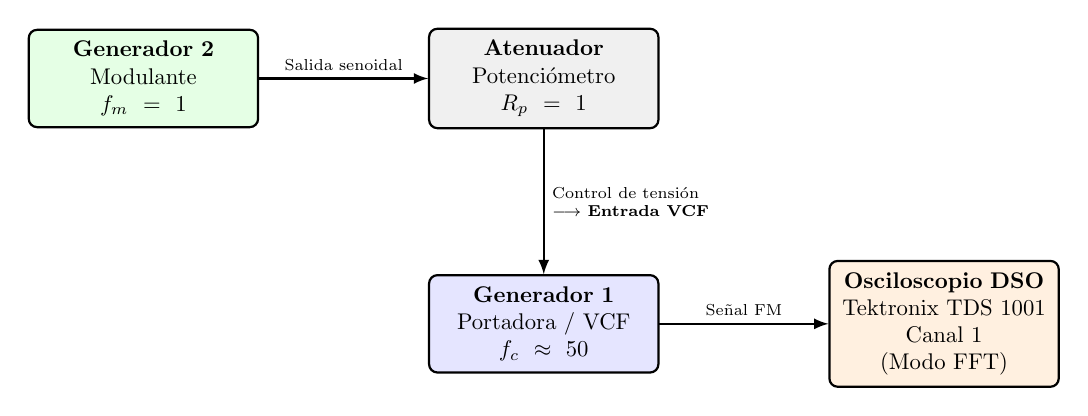
\begin{tikzpicture}[scale=0.82, transform shape,
    block/.style={rectangle, draw, fill=blue!8, rounded corners=3pt, thick, 
                  text width=3.2cm, text centered, minimum height=1.5cm, inner sep=5pt},
    line/.style={draw, -latex, thick}
]
    % Fila superior: Generador 2 (Modulante) y Potenciómetro Atenuador
    \node[block, fill=green!10] (g2) at (0, 2.2) {
        \textbf{Generador 2}\\Modulante\\$f_m = \qty{1}{\kilo\hertz}$
    };

    \node[block, fill=gray!12] (pot) at (6.2, 2.2) {
        \textbf{Atenuador}\\Potenciómetro\\$R_p = \qty{1}{\kilo\ohm}$
    };

    % Fila inferior: Generador 1 (Portadora y entrada VCF) y Osciloscopio Digital DSO
    \node[block, fill=blue!10] (g1) at (6.2, -1.6) {
        \textbf{Generador 1}\\Portadora / VCF\\$f_c \approx \qty{50}{\kilo\hertz}$
    };

    \node[block, fill=orange!12, text width=3.2cm] (osc) at (12.4, -1.6) {
        \textbf{Osciloscopio DSO}\\Tektronix TDS 1001\\Canal 1 (Modo FFT)
    };

    % Conexiones con etiquetas claras y sin superposiciones
    \path[line] (g2.east) -- node[above, font=\scriptsize] {Salida senoidal} (pot.west);
    \path[line] (pot.south) -- node[right, font=\scriptsize, align=left] {Control de tensión\\$\longrightarrow$ \textbf{Entrada VCF}} (g1.north);
    \path[line] (g1.east) -- node[above, font=\scriptsize] {Señal FM} (osc.west);
\end{tikzpicture}

    \caption{Diagrama de interconexión para modulación FM mediante entrada de control VCF.}
    \label{crkt.ej6:conexion_fm}
\end{figure}

Se dispuso:
\begin{itemize}
    \item $G_1$ (Portadora): senoidal de $f_c \approx \qty{50}{\kilo\hertz}$ (ajustada en $\qty{49.7}{\kilo\hertz}$).
    \item $G_2$ (Modulante): senoidal de $f_m = \qty{1}{\kilo\hertz}$.
\end{itemize}
Con la base de tiempos en $\qty{1}{\milli\second\per\text{div}}$ se apreció la superposición de trazos debida a la modulación
en frecuencia. En el \texttt{Math Menú} se seleccionó FFT en CH1, ventana Hanning, Zoom X10 y Promedio de 64 cuentas.

Con los cursores en Frecuencia se registraron los valores:
\begin{itemize}
    \item Frecuencia portadora (Port): $\qty{49.7}{\kilo\hertz}$.
    \item Frecuencia lateral sup/inf (FL\_): $\qty{50.7}{\kilo\hertz} \text{ / } \qty{48.7}{\kilo\hertz}$.
    \item Frecuencia modulante ($\text{Dif.} = \text{FLS} - f_c$): $\qty{1}{\kilo\hertz}$.
\end{itemize}

\subsection{Observaciones y Anulación de Portadora}
Siguiendo las pautas de la consigna:
\begin{itemize}
    \item Al variar el nivel de la señal modulante con el potenciómetro atenuador, se observó cómo se modificaba la
    amplitud de la portadora y aparecían más bandas laterales a medida que crecía el índice de modulación.
    \item Se buscó experimentalmente el valor de modulación que anuló por completo la portadora central en la pantalla
    del osciloscopio (Figura~\ref{fig.ej6:foto_anulacion}), condición correspondiente a un índice de modulación
    $\beta = 2{,}4$.
    \item Se conmutó la modulante a forma cuadrada (Figura~\ref{fig.ej6:fm_cuadrada}) y triangular
    (Figura~\ref{fig.ej6:fm_triangular}), apreciando los espectros correspondientes.
    \item Se contrastaron las ventanas Flattop (Figura~\ref{fig.ej6:fm_flattop}) y Rectangular
    (Figura~\ref{fig.ej6:fm_rectangular}).
\end{itemize}

\begin{figure}[!ht]
    \centering
    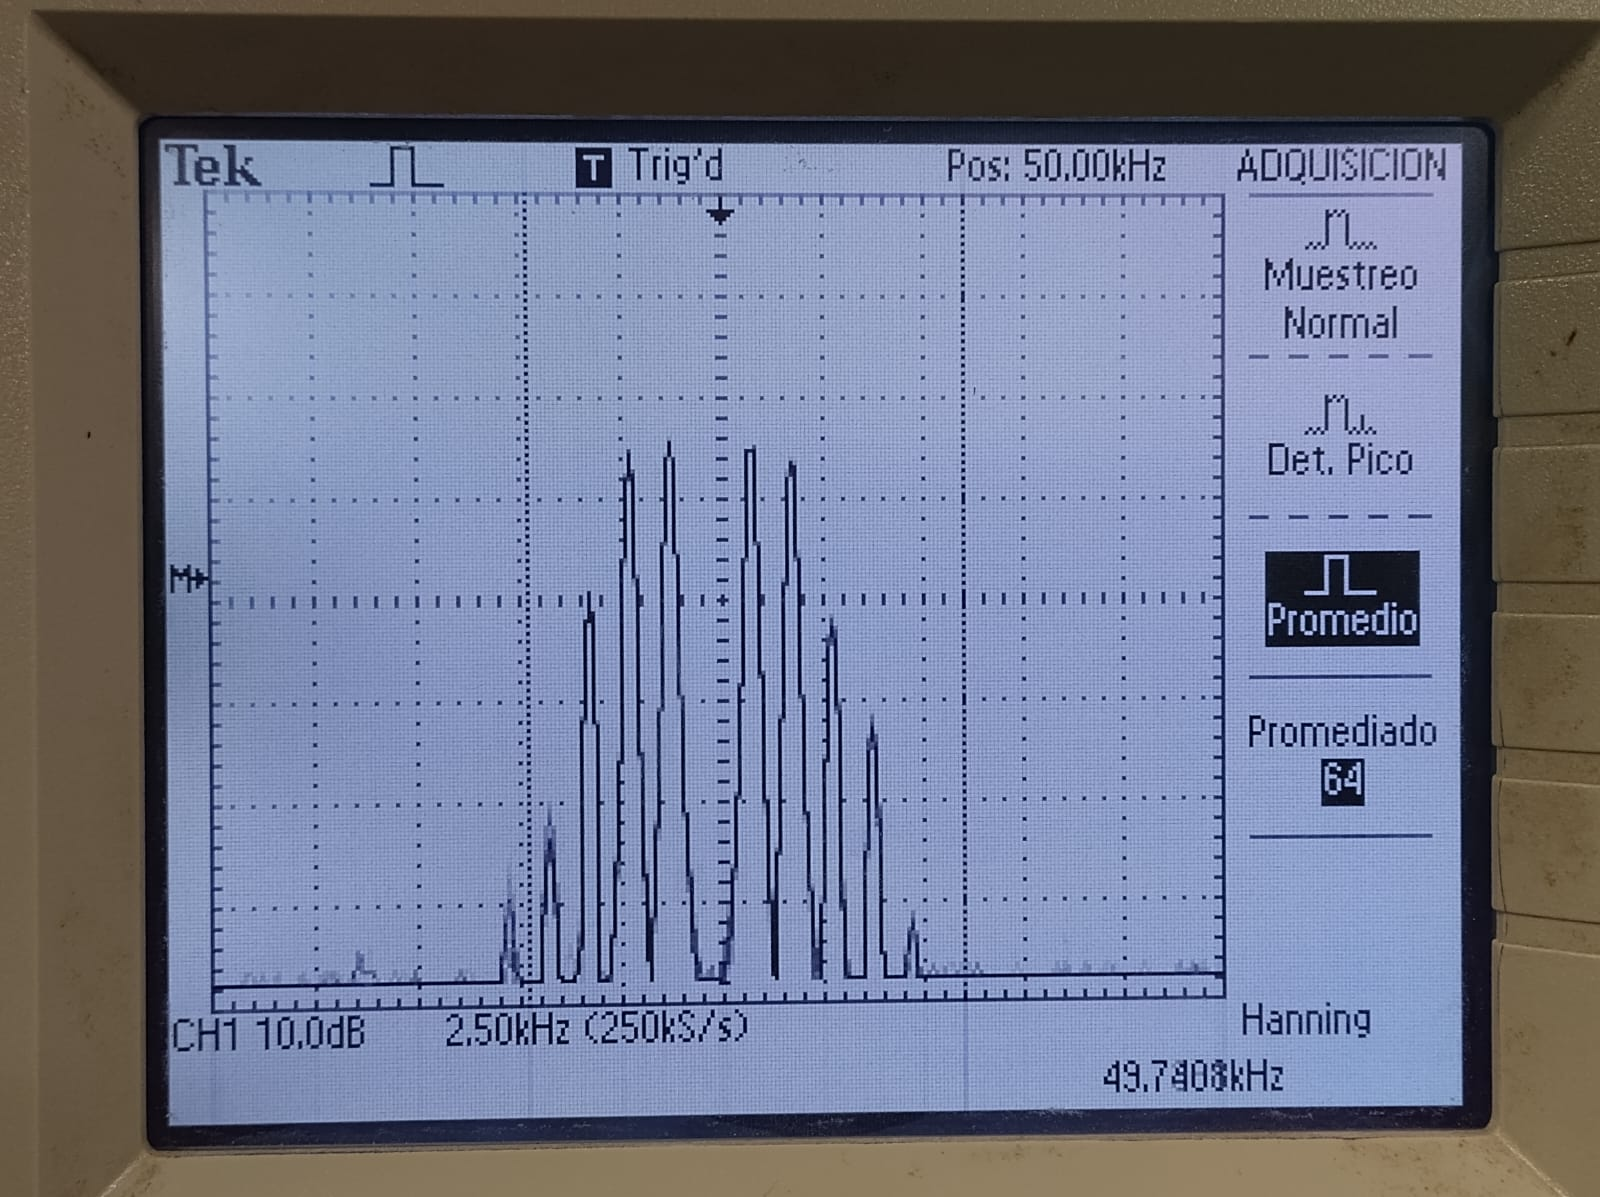
\includegraphics[width=0.46\textwidth]{pictures/foto13.jpg}
    \caption{Espectro FM en la condición de portadora anulada ($\beta = 2{,}4$).}
    \label{fig.ej6:foto_anulacion}
\end{figure}

\begin{figure}[!ht]
    \centering
    \begin{subfigure}[t]{0.48\textwidth}
        \centering
        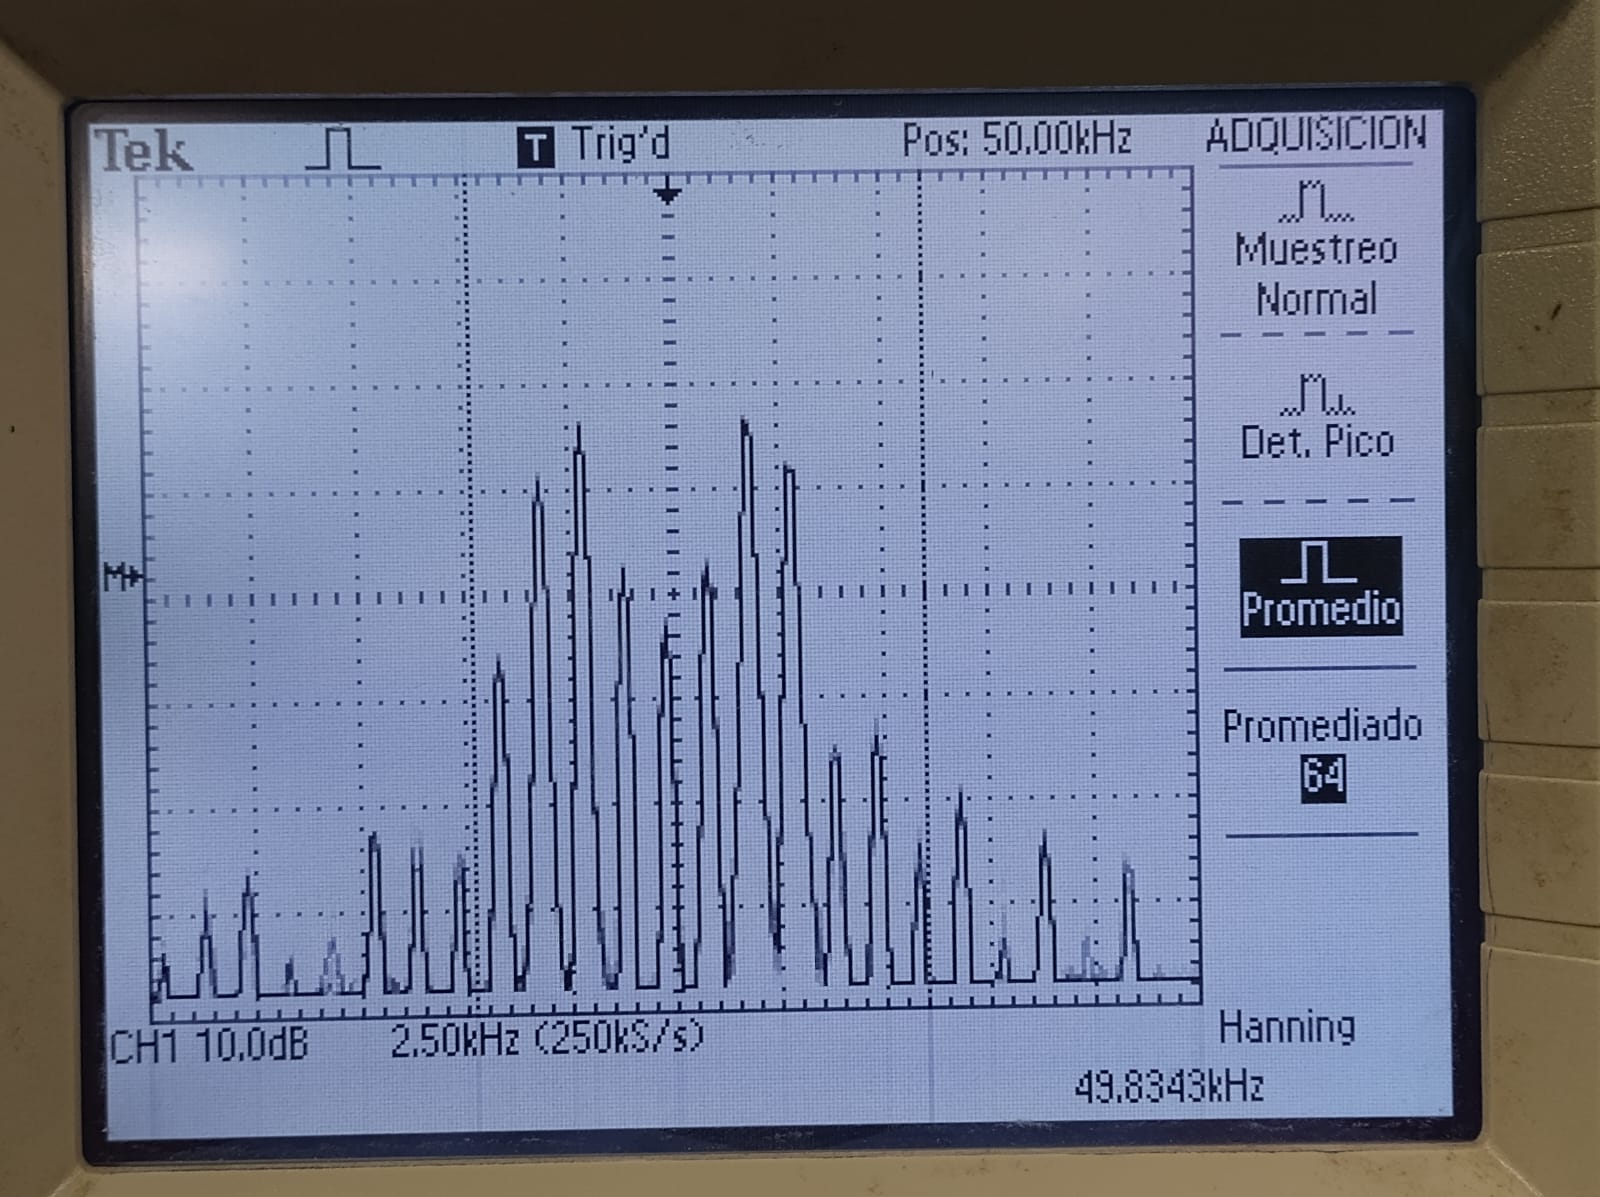
\includegraphics[width=\textwidth]{pictures/foto14.jpg}
        \caption{Modulante cuadrada.}
        \label{fig.ej6:fm_cuadrada}
    \end{subfigure}
    \hfill
    \begin{subfigure}[t]{0.48\textwidth}
        \centering
        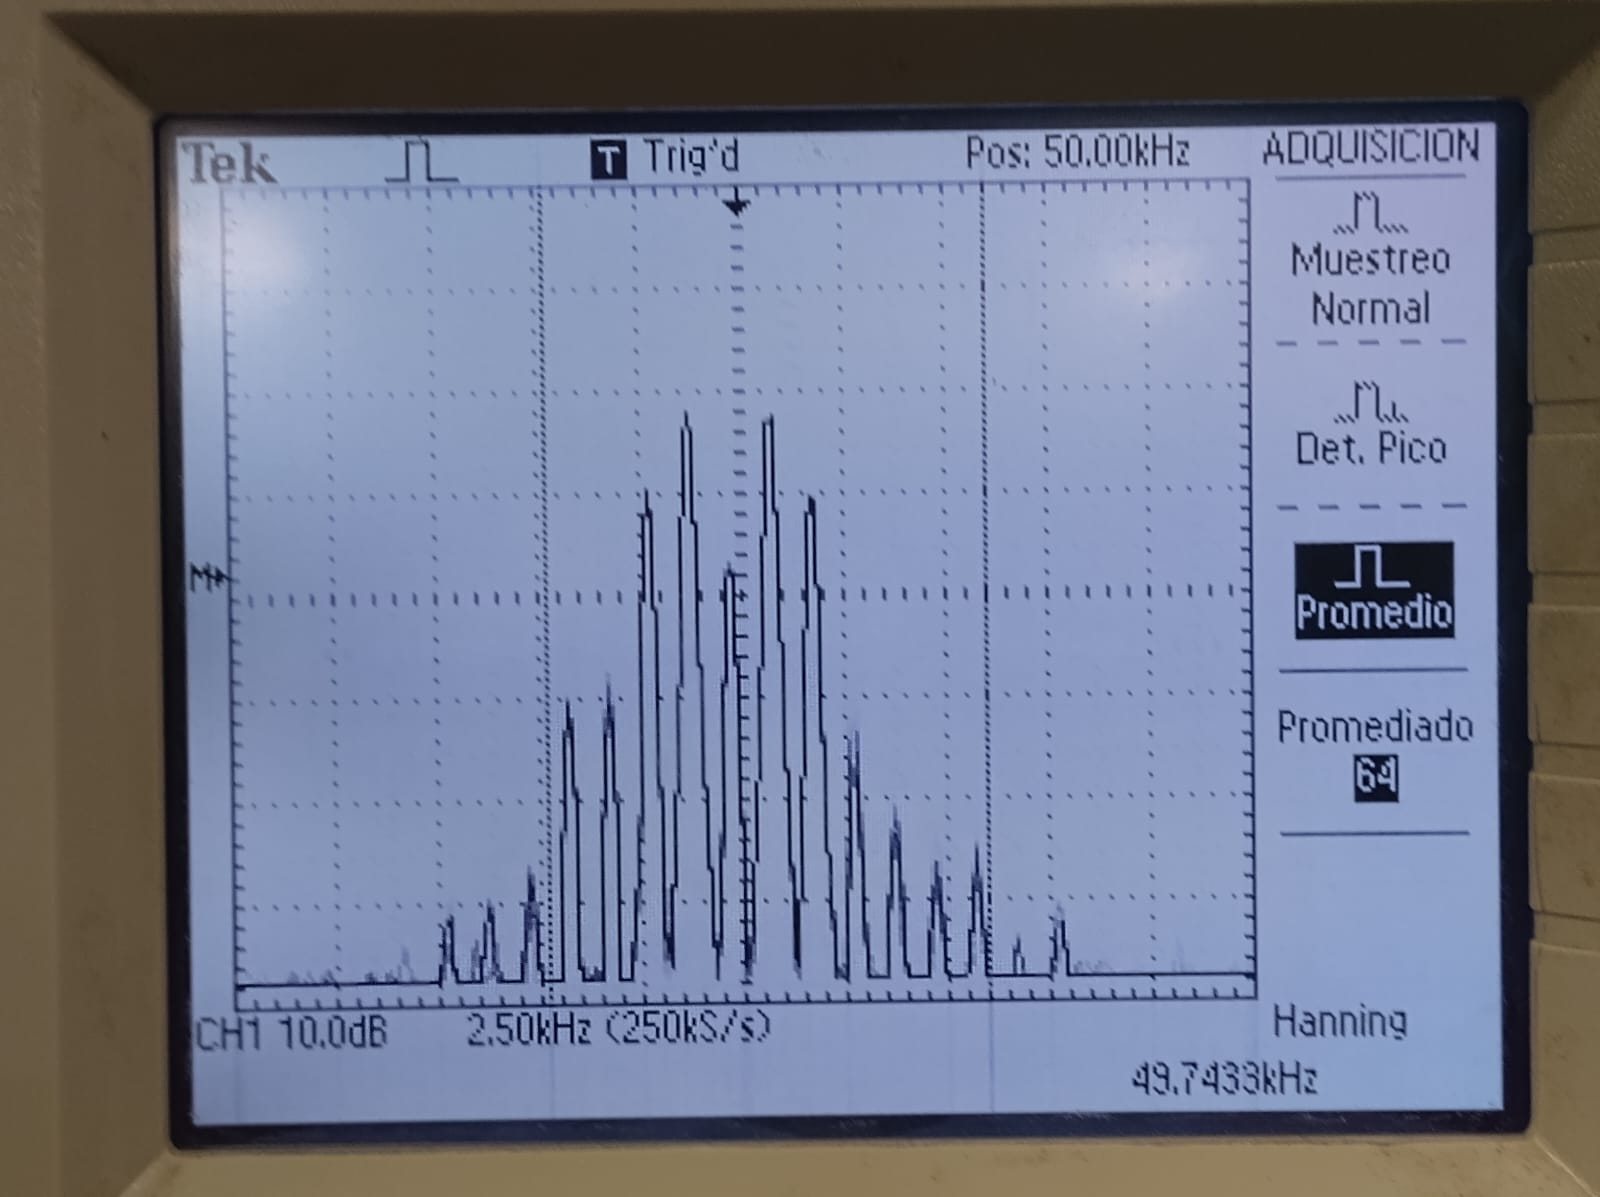
\includegraphics[width=\textwidth]{pictures/foto15.jpg}
        \caption{Modulante triangular.}
        \label{fig.ej6:fm_triangular}
    \end{subfigure}
    \caption{Espectros de frecuencia modulada con modulantes cuadrada y triangular.}
    \label{fig.ej6:fm_modulantes}
\end{figure}

\begin{figure}[!ht]
    \centering
    \begin{subfigure}[t]{0.48\textwidth}
        \centering
        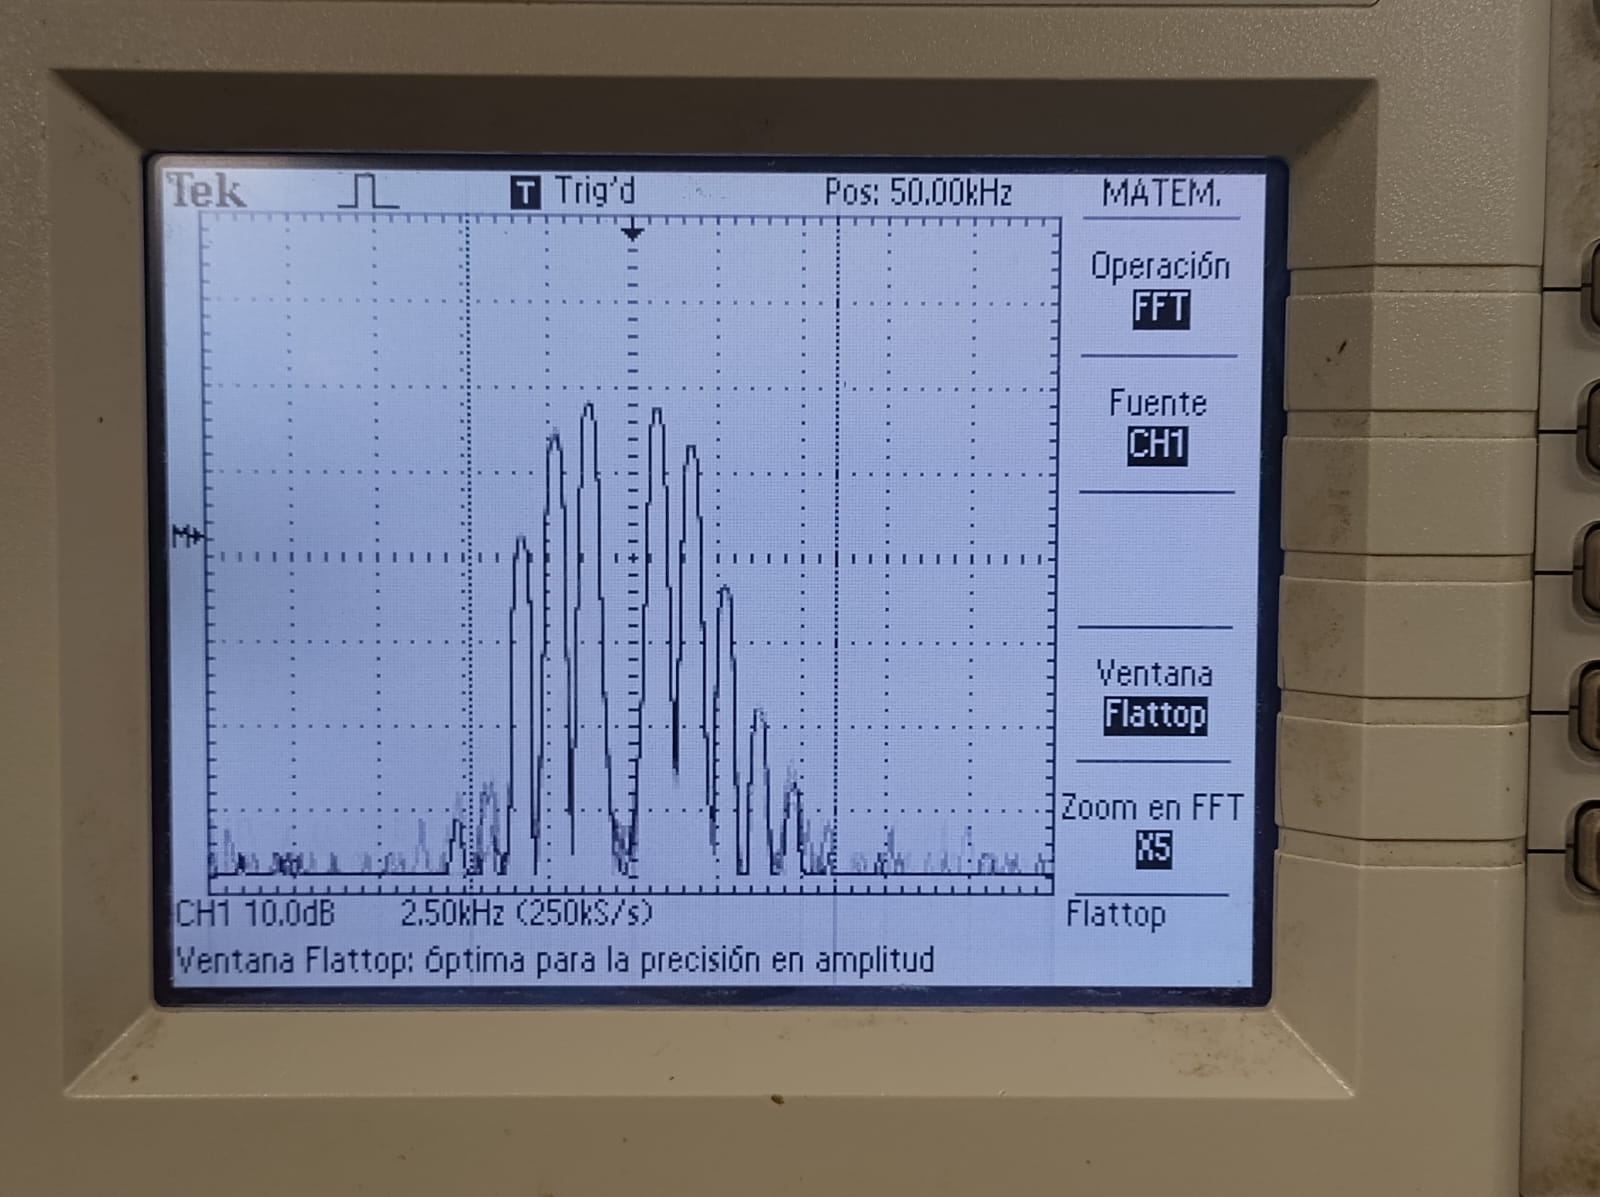
\includegraphics[width=\textwidth]{pictures/foto16.jpg}
        \caption{Ventana Flattop.}
        \label{fig.ej6:fm_flattop}
    \end{subfigure}
    \hfill
    \begin{subfigure}[t]{0.48\textwidth}
        \centering
        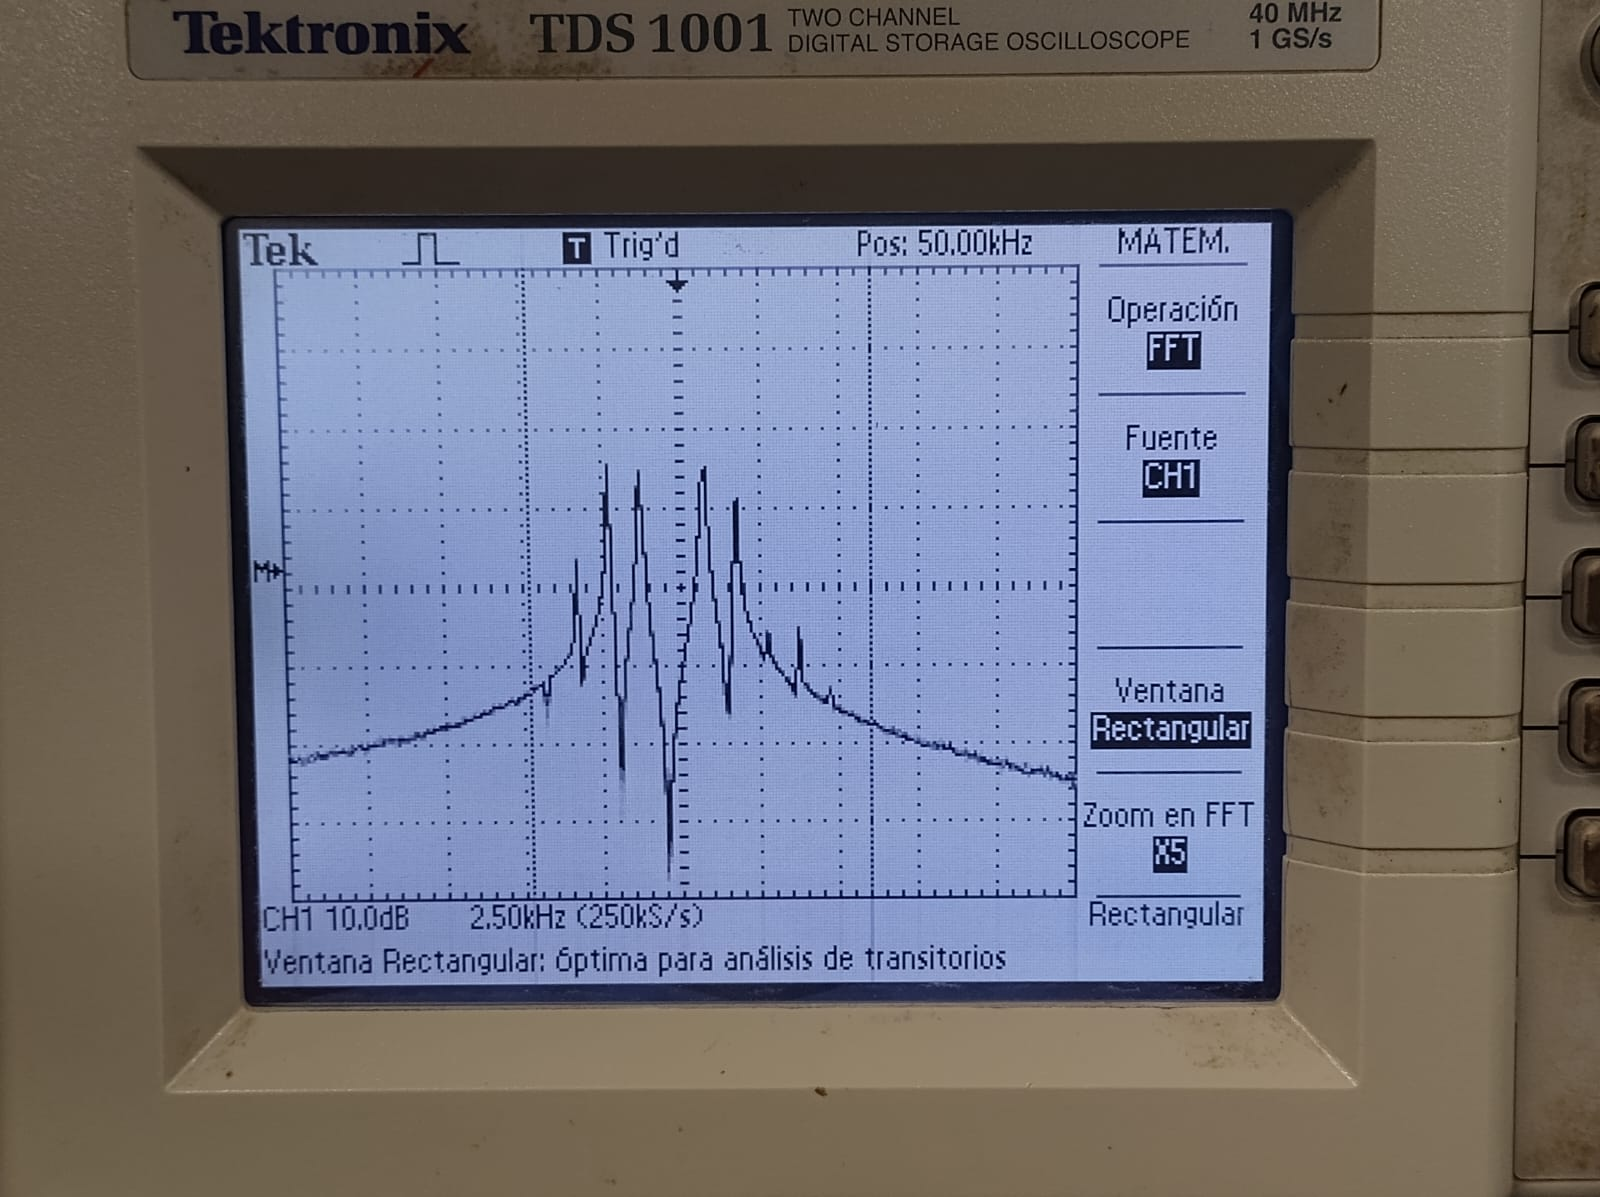
\includegraphics[width=\textwidth]{pictures/foto17.jpg}
        \caption{Ventana Rectangular.}
        \label{fig.ej6:fm_rectangular}
    \end{subfigure}
    \caption{Comparación de ventanas en la medición del espectro de frecuencia modulada.}
    \label{fig.ej6:ventanas_fm}
\end{figure}

% =========================================================================
% EXPERIMENTO 7
% =========================================================================
\section{Experimento 7: Medición de Distorsión Armónica en Amplificador}
\label{sec.ej7:distorsion_armonica}

\subsection{Procedimiento y Circuito de Medición}
Se empleó el módulo de amplificador transistorizado de dos etapas (clase A). La medición se efectuó sin carga conectada
(funcionamiento como amplificador de tensión pura), conectando el instrumental según el esquema de la
Figura~2 de la consigna (reproducido en la Figura~\ref{crkt.ej7:medicion_thd}).

\begin{figure}[!ht]
    \centering
    % Circuito esquemático de medición de distorsión armónica en un amplificador (Figura 2 de la consigna)
\begin{tikzpicture}[scale=0.85, transform shape,
    block/.style={rectangle, draw, rounded corners=3pt, thick, 
                  text centered, minimum height=1.6cm, inner sep=6pt},
    line/.style={draw, thick}
]
    % 1. Bloque Generador BF
    \node[block, fill=blue!5, text width=2.6cm] (gen) at (0, 0) {
        \textbf{Generador BF}\\(\qty{1}{\kilo\hertz})
    };
    \draw (gen.south) to[short] ++(0,-0.4) node[ground] {};

    % 2. Bloque Amplificador de 2 etapas
    \node[block, fill=green!8, text width=3.8cm] (amp) at (5.2, 0) {
        \textbf{Amplificador 2 etapas}\\[2pt]
        {\scriptsize (Lazo Abierto / Lazo Cerrado)}\\[2pt]
        {\tiny Módulo experimental}
    };
    \draw (amp.south) to[short] ++(0,-0.4) node[ground] {};

    % 3. Bloque Osciloscopio con FFT
    \node[block, fill=blue!3, text width=3.2cm] (osc) at (12.0, 0) {
        \textbf{Osciloscopio DSO}\\[2pt]
        {\scriptsize Modo FFT (Flattop)}\\[2pt]
        {\tiny Medición armónicos $V_1, V_2, V_3$}
    };
    \draw (osc.south) to[short] ++(0,-0.4) node[ground] {};

    % 4. Bloque Voltímetro True RMS (opcional)
    \node[block, fill=purple!5, text width=2.8cm, minimum height=1.3cm] (volt) at (8.6, -2.4) {
        \textbf{Voltímetro True RMS}\\[2pt]
        {\tiny UNI-T UT89X ($V_{\text{ef}}$)}
    };
    \draw (volt.south) to[short] ++(0,-0.4) node[ground] {};

    % Conexión Generador -> Amplificador
    \draw[line] (gen.east) to[short, -o] ++(0.4,0);
    \draw[line] (amp.west) to[short, -o] ++(-0.4,0);
    \draw[line] ([xshift=0.4cm]gen.east) -- node[above, font=\scriptsize] {Entrada} ([xshift=-0.4cm]amp.west);

    % Conexión Amplificador -> Nodo de distribución
    \draw[line] (amp.east) to[short, -o] ++(0.4,0);
    \node at ([xshift=0.4cm, yshift=0.3cm]amp.east) [font=\scriptsize] {Salida};
    
    % Nodo de distribución a x=8.6
    \draw[line] ([xshift=0.4cm]amp.east) -- (8.6, 0) node[circle, fill, inner sep=1.5pt] {};

    % Derivación vertical hacia el Voltímetro
    \draw[line] (8.6, 0) -- (8.6, -1.3)
        to[short, -o] (8.6, -1.5)
        -- (volt.north);

    % Conexión hacia el Osciloscopio
    \draw[line] (8.6, 0) -- ([xshift=-0.6cm]osc.west)
        to[short, -o] ([xshift=-0.2cm]osc.west) node[above left, font=\scriptsize\bfseries] {CH1}
        -- (osc.west);
\end{tikzpicture}

    \caption{Circuito de medición de distorsión armónica en amplificador (Figura 2 de la consigna).}
    \label{crkt.ej7:medicion_thd}
\end{figure}

Se dispusieron los jumpers correspondientes para que el circuito operara inicialmente a \emph{lazo abierto}.
En el osciloscopio se activó la reducción de ancho de banda a $\qty{20}{\mega\hertz}$ para evitar posibles frecuencias alias.
Se aplicó una señal senoidal de $\qty{1}{\kilo\hertz}$ ajustando el generador para alcanzar la máxima excursión simétrica
sin recorte en la salida, registrándose en el dominio del tiempo una tensión de salida de $\qty{6.56}{\volt_{pap}}$
(Figura~\ref{fig.ej7:tiempo_abierto}).

\begin{figure}[!ht]
    \centering
    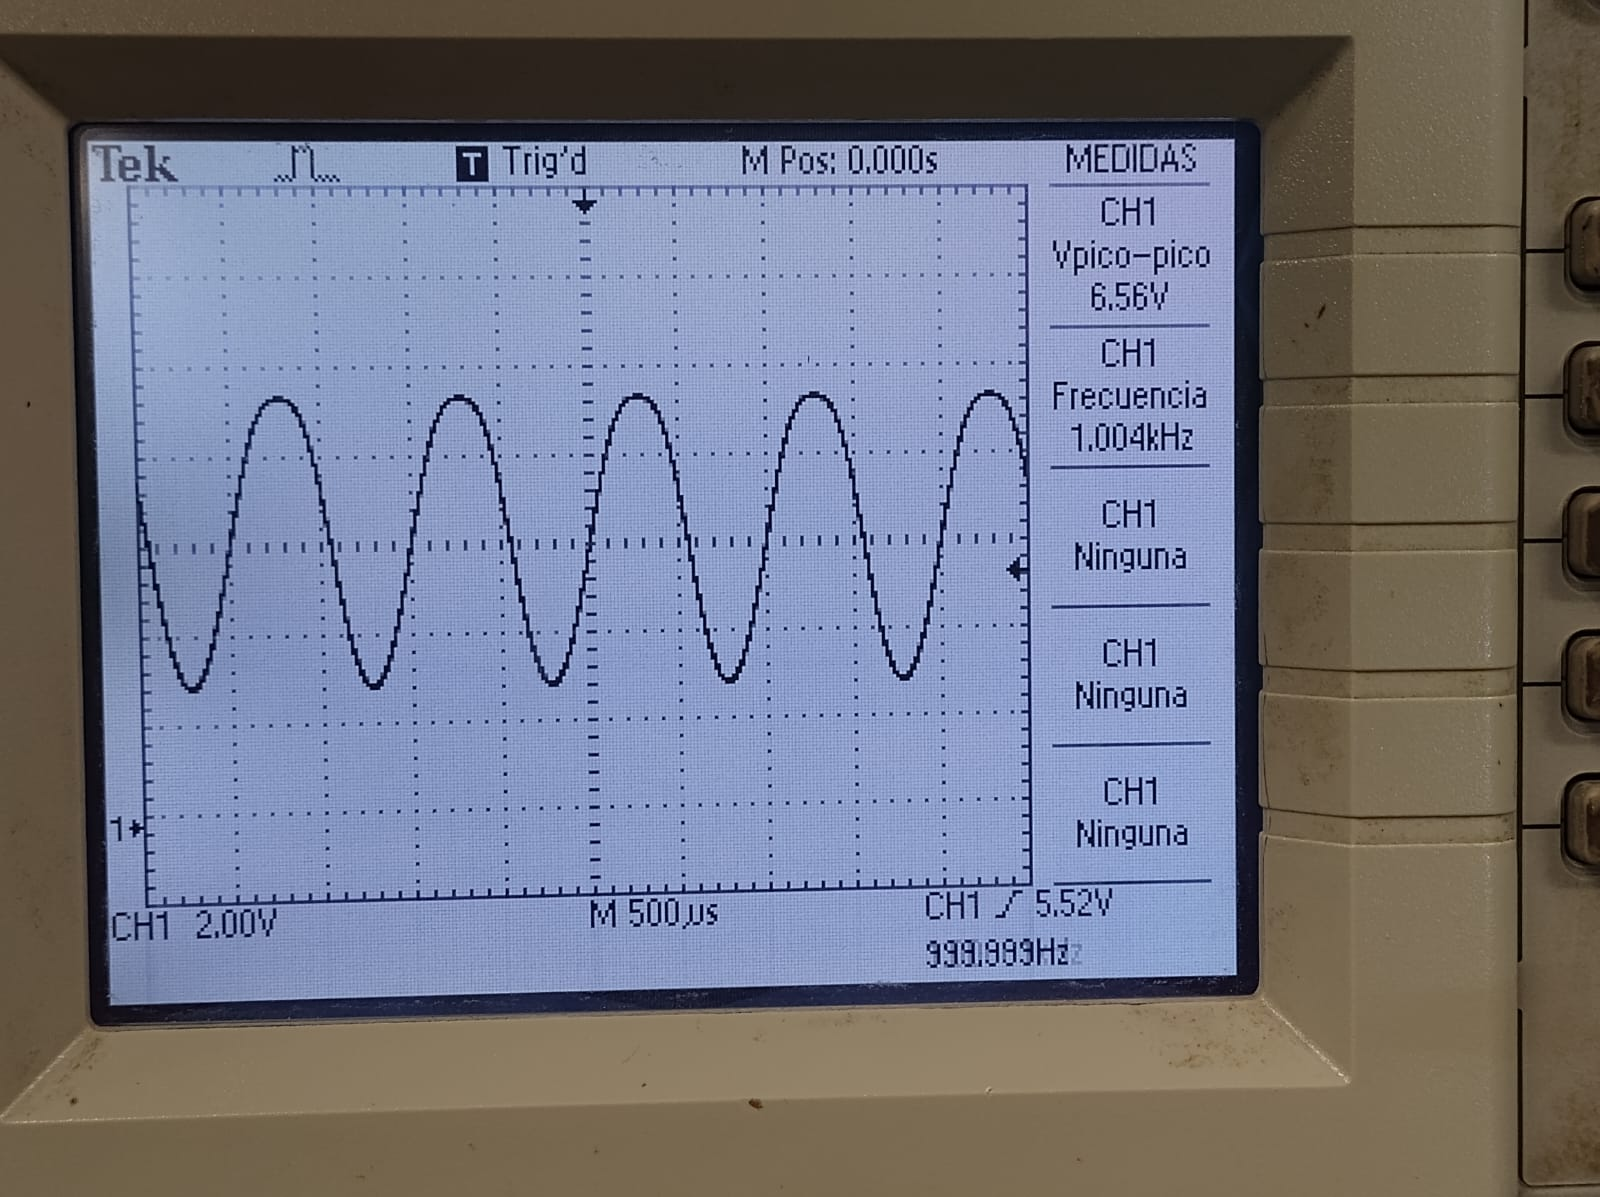
\includegraphics[width=0.46\textwidth]{pictures/foto18.jpg}
    \caption{Señal de salida a lazo abierto en el dominio del tiempo ($\qty{6.56}{\volt_{pap}}$).}
    \label{fig.ej7:tiempo_abierto}
\end{figure}

\subsection{Mediciones a Lazo Abierto}
Se conmutó el osciloscopio al modo FFT con ventana Flattop y Zoom X10 (Figura~\ref{fig.ej7:fft_abierto}), determinando
las frecuencias y amplitudes de la fundamental y de los armónicos 2° y 3°. Se completó la tabla de la consigna según
se detalla en el Cuadro~\ref{tab.ej7:lazo_abierto}.

\begin{figure}[!ht]
    \centering
    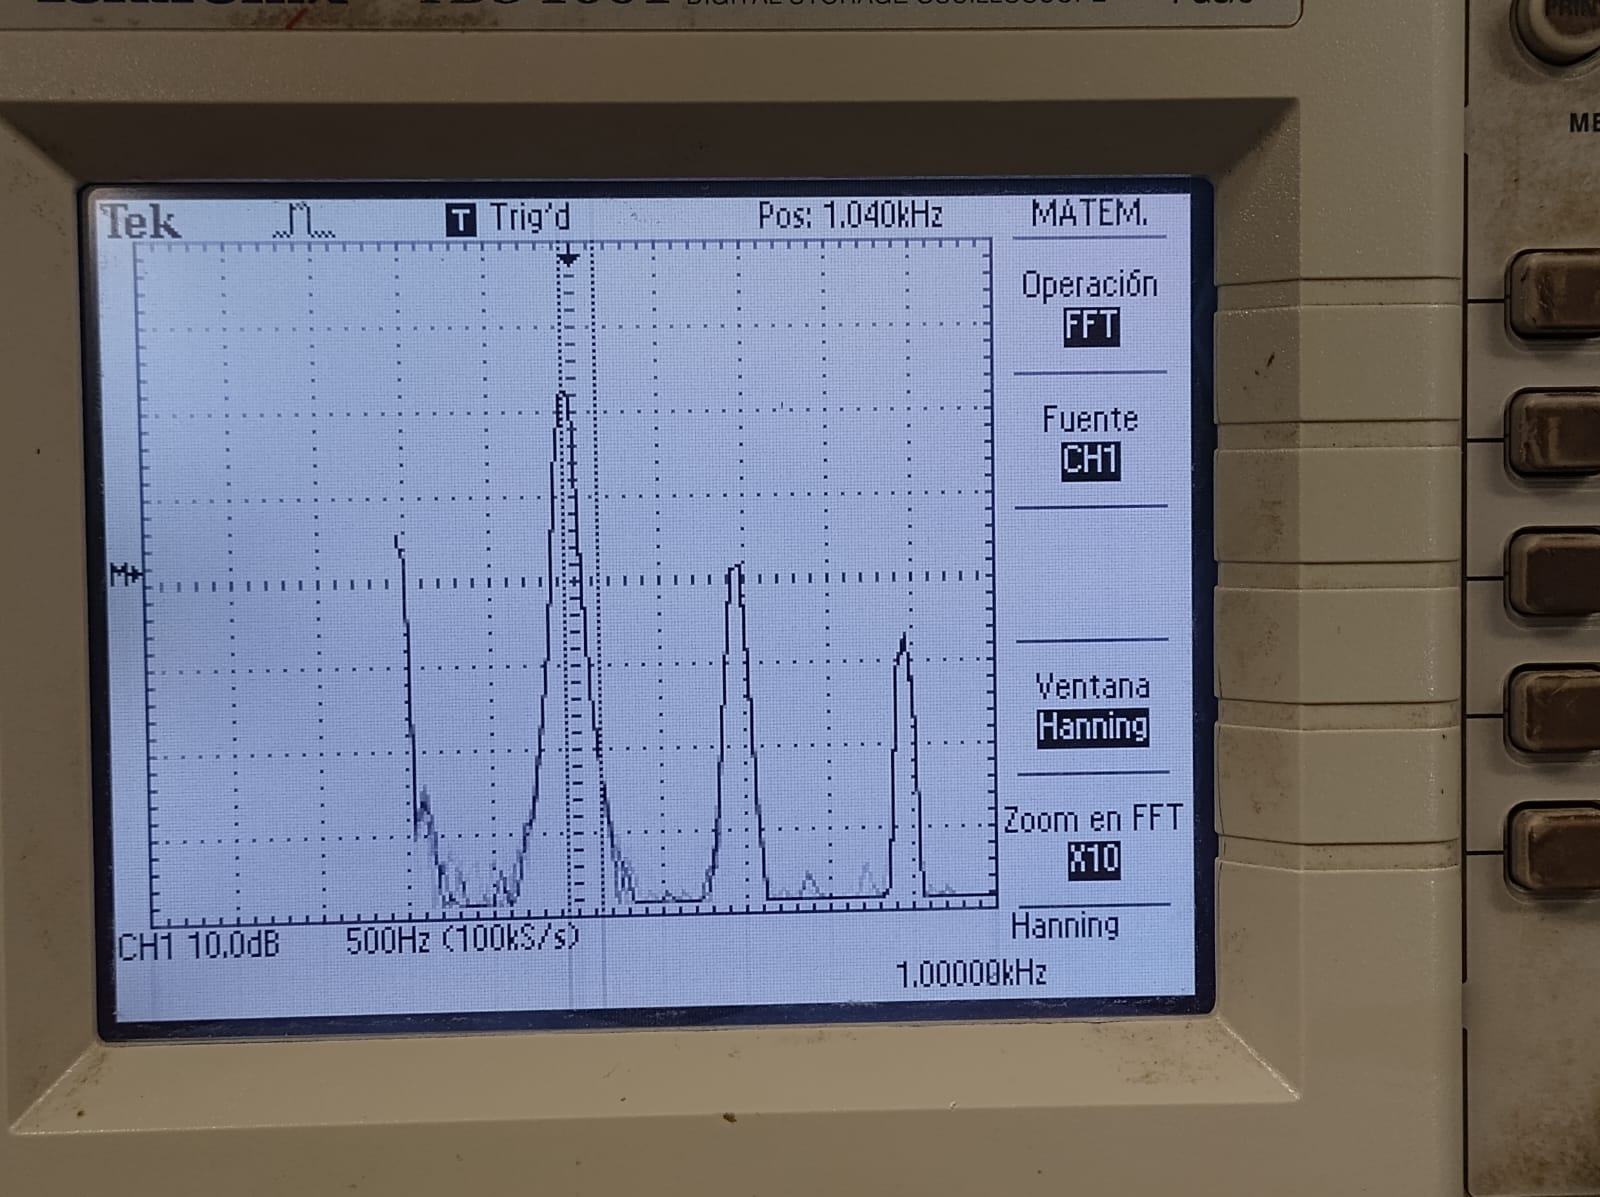
\includegraphics[width=0.46\textwidth]{pictures/foto19.jpg}
    \caption{Espectro FFT a lazo abierto con componentes de 1ra, 2da y 3ra armónica.}
    \label{fig.ej7:fft_abierto}
\end{figure}

\begin{table}[!ht]
    \centering
    \resizebox{\textwidth}{!}{%
    \begin{tabular}{lcccc}
        \toprule
        & \textbf{En el dominio del tiempo} & \multicolumn{3}{c}{\textbf{En el dominio de la frecuencia (FFT)}} \\
        \cmidrule(lr){2-2} \cmidrule(lr){3-5}
        & $V_{\text{salida}}\ [V_{\text{pap}}]$ & $V_1$ (1er Armónica) & $V_2$ (2da Armónica) & $V_3$ (3ra Armónica) \\
        \midrule
        \textbf{Frec (kHz)} & $\qty{1}{\kilo\hertz}$ & $\qty{1}{\kilo\hertz}$ & $\qty{2}{\kilo\hertz}$ & $\qty{3}{\kilo\hertz}$ \\
        \textbf{dBv} & ------- & $+7{,}85$ & $-13{,}7$ & $-22{,}9$ \\
        \textbf{V [$\unit{\volt_{rms}}$]} & $\qty{6.56}{\volt_{pap}}$ & $\qty{2.47}{\volt}$ & $\qty{0.207}{\volt}$ & $\qty{0.0716}{\volt}$ \\
        \bottomrule
    \end{tabular}}
    \caption{Tabla de valores medidos a lazo abierto (estructura oficial de la consigna).}
    \label{tab.ej7:lazo_abierto}
\end{table}

A partir de los valores medidos, se calculó la tensión armónica eficaz y el porcentaje de distorsión armónica mediante
las expresiones consignadas:
\begin{equation}
    V(\text{Arm.}) = \sqrt{V_2^2 + V_3^2} = \sqrt{(0{,}207)^2 + (0{,}0716)^2} = \qty{0.219}{\volt}
    \label{eq.ej7:varm_abierto}
\end{equation}
\begin{equation}
    \text{Dist.Arm.\%} = \frac{V(\text{Arm})}{V_1} \cdot 100 = \frac{0{,}219}{2{,}47} \cdot 100 = 8{,}85\%
    \label{eq.ej7:thd_abierto}
\end{equation}
\begin{equation*}
    \textbf{Distorsión Armónica \% (a lazo abierto)} = \mathbf{8{,}85\%}
\end{equation*}

\subsection{Mediciones a Lazo Cerrado}
Sin desconectar los instrumentos, se insertó el jumper para activar el lazo de realimentación negativa.
Tal como se preveía, el nivel de salida cayó sensiblemente por la disminución de ganancia del amplificador.
En el espectro FFT (Figura~\ref{fig.ej7:fft_cerrado}) se adquirió la respuesta a lazo cerrado, registrándose una
fundamental atenuada a $-16{,}9\,\unit{\dBV}$ ($142{,}9\,\unit{\milli\volt_{rms}}$, correspondiente a una tensión temporal
reducida a $\approx \qty{0.40}{\volt_{pap}}$). Se completó la tabla de la consigna (Cuadro~\ref{tab.ej7:lazo_cerrado}).

\begin{figure}[!ht]
    \centering
    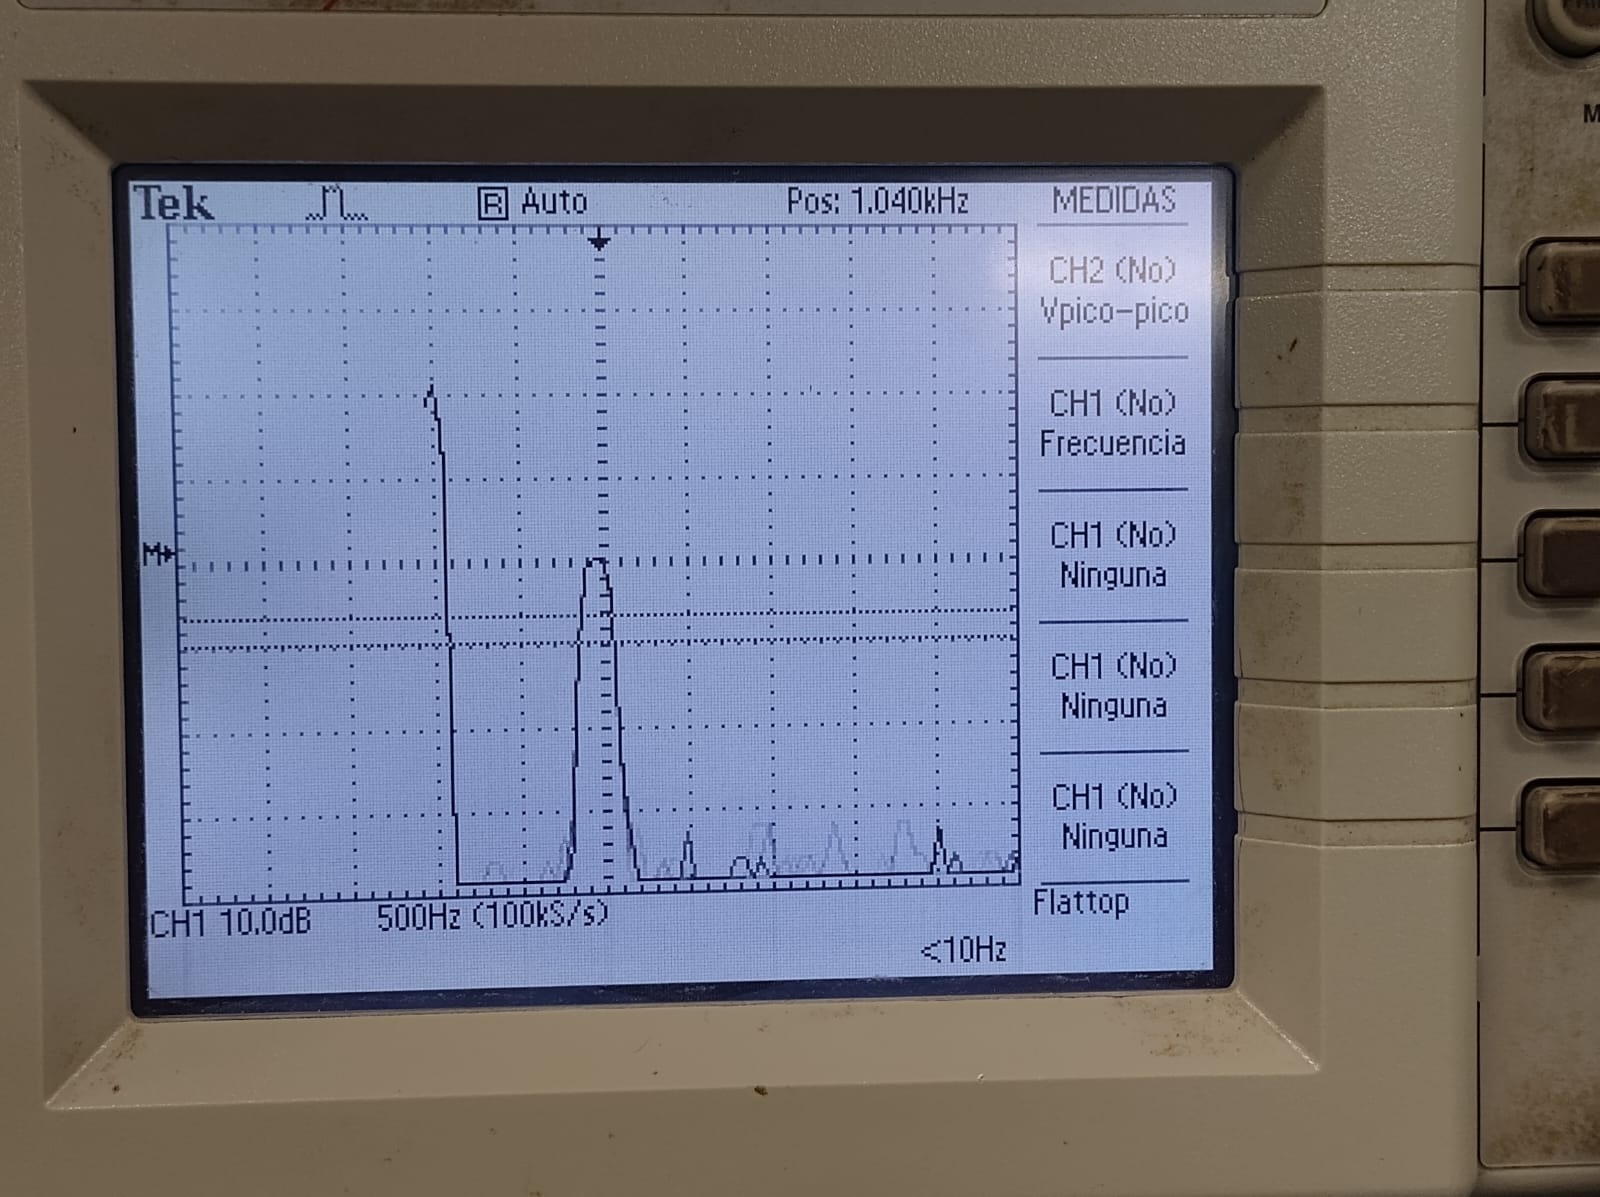
\includegraphics[width=0.46\textwidth]{pictures/foto20.jpg}
    \caption{Espectro FFT del amplificador a lazo cerrado con reducción de armónicos.}
    \label{fig.ej7:fft_cerrado}
\end{figure}

\begin{table}[!ht]
    \centering
    \resizebox{\textwidth}{!}{%
    \begin{tabular}{lcccc}
        \toprule
        & \textbf{En el dominio del tiempo} & \multicolumn{3}{c}{\textbf{En el dominio de la frecuencia (FFT)}} \\
        \cmidrule(lr){2-2} \cmidrule(lr){3-5}
        & $V_{\text{salida}}\ [V_{\text{pap}}]$ & $V_1$ (1er Armónica) & $V_2$ (2da Armónica) & $V_3$ (3ra Armónica) \\
        \midrule
        \textbf{Frec (kHz)} & $\qty{1}{\kilo\hertz}$ & $\qty{1}{\kilo\hertz}$ & $\qty{2}{\kilo\hertz}$ & $\qty{3}{\kilo\hertz}$ \\
        \textbf{dBv} & ------- & $-16{,}9$ & $-43{,}9$ & $-44{,}9$ \\
        \textbf{V [$\unit{\volt_{rms}}$]} & $\qty{0.40}{\volt_{pap}}$ & $\qty{0.143}{\volt}$ & $\qty{0.00638}{\volt}$ & $\qty{0.00569}{\volt}$ \\
        \bottomrule
    \end{tabular}}
    \caption{Tabla de valores medidos a lazo cerrado (estructura oficial de la consigna).}
    \label{tab.ej7:lazo_cerrado}
\end{table}

Calculando la distorsión armónica a lazo cerrado:
\begin{equation}
    V(\text{Arm.}) = \sqrt{V_2^2 + V_3^2} = \sqrt{(0{,}00638)^2 + (0{,}00569)^2} = \qty{0.00855}{\volt}
    \label{eq.ej7:varm_cerrado}
\end{equation}
\begin{equation}
    \text{Dist.Arm.\%} = \frac{V(\text{Arm})}{V_1} \cdot 100 = \frac{0{,}00855}{0{,}143} \cdot 100 = 5{,}98\%
    \label{eq.ej7:thd_cerrado}
\end{equation}
\begin{equation*}
    \textbf{Distorsión Armónica \% (a lazo cerrado)} = \mathbf{5{,}98\%}
\end{equation*}

\subsection{Comparación entre Lazo Abierto y Lazo Cerrado}
Al comparar los valores obtenidos en ambos pasos según lo solicitado en el inciso~(l) de la consigna:
\begin{itemize}
    \item A lazo abierto, operando en máxima excursión, el amplificador ingresó en zonas no lineales de su curva de
    transferencia, registrando una distorsión armónica del $8{,}85\%$.
    \item A lazo cerrado, la realimentación negativa aumentó la linealidad global del circuito, atenuando los armónicos
    segundo y tercero en mayor proporción que la fundamental y reduciendo el porcentaje de distorsión armónica al $5{,}98\%$.
\end{itemize}
